\documentclass[11pt]{article}
\usepackage[utf8]{inputenc}
\usepackage[T1]{fontenc}
\usepackage{amsmath,amssymb,graphicx,url,tabularx,booktabs,float}
\usepackage[margin=1in]{geometry}
\renewcommand{\thefigure}{S\arabic{figure}}
\renewcommand{\thetable}{S\arabic{table}}
\title{Supplementary Material for ``Back-Surface-Field-Enhanced, Defect-and-Optics-Budgeted Design of Lead-Free RbGeI$_{3}$/CuI Solar Cells''}
\author{Md.\ Abdul Malek Fahim and Hussain Touhid Siddiquee}
\begin{document}
\maketitle

\section*{S1.\ One-at-a-time sweep details}
Full per-parameter traces for the eleven sequential optimization steps summarized in Section~2 of the main text (baseline campaign; consolidated device 26.81\%).

\subsection*{Absorber thickness (Fig.~S1)}
PCE peaks at 0.7\,$\mu$m (20.70\%); $J_{\mathrm{SC}}$ climbs 28.14$\rightarrow$34.11\,mA/cm$^{2}$ while $V_{\mathrm{OC}}$ slides 0.823$\rightarrow$0.767\,V. The upper $J_{\mathrm{SC}}$ readings come from the early Step-1 deck with extended sub-gap absorption; re-simulation on the consolidated uniform-1.4\,eV deck gives 25.2--31.3\,mA/cm$^{2}$ with the same peak-plateau shape, so 0.7\,$\mu$m stands.
\begin{figure}[H]\centering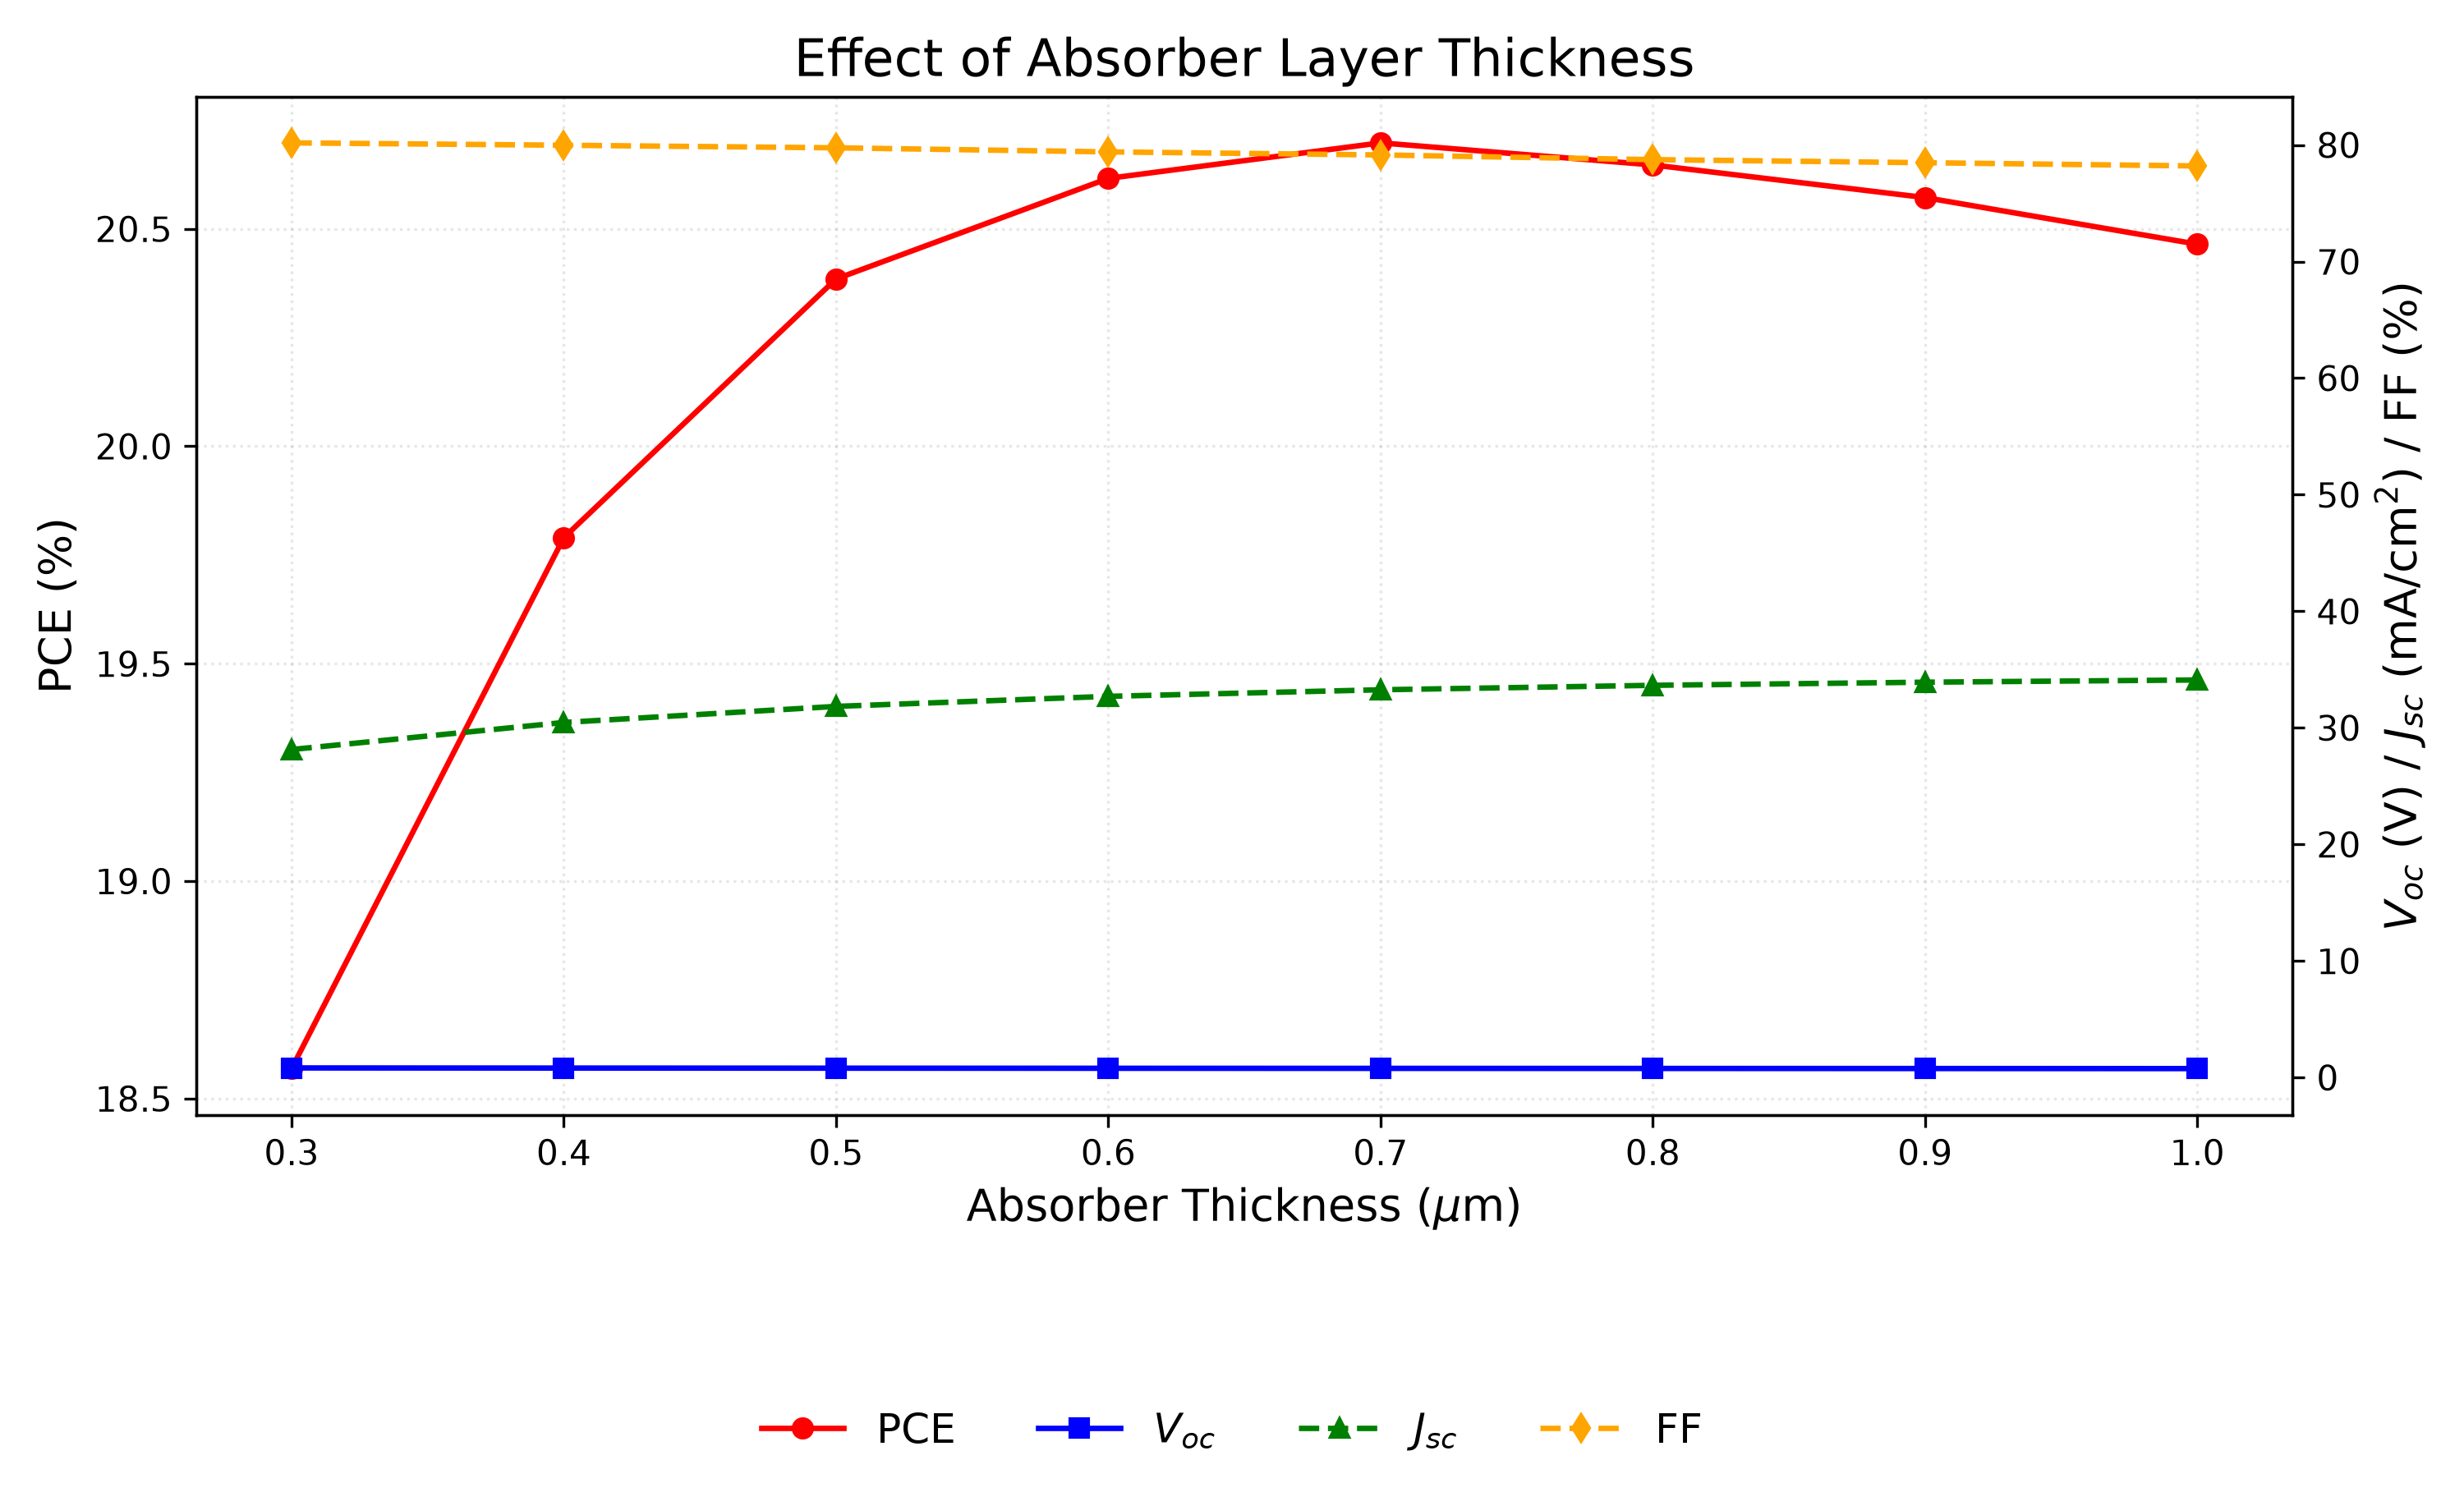
\includegraphics[width=0.85\linewidth]{figs/sup_fig3.png}
\caption{Fig.~S1: PCE, $V_{\mathrm{OC}}$, $J_{\mathrm{SC}}$, FF vs absorber thickness.}\end{figure}

\subsection*{Dielectric constant (Fig.~S2)}
Raising $\epsilon_{r}$ 15$\rightarrow$23.1 moves PCE 19.92$\rightarrow$19.79\% via $V_{\mathrm{OC}}$ only; $\epsilon_{r}=15$ kept.
\begin{figure}[H]\centering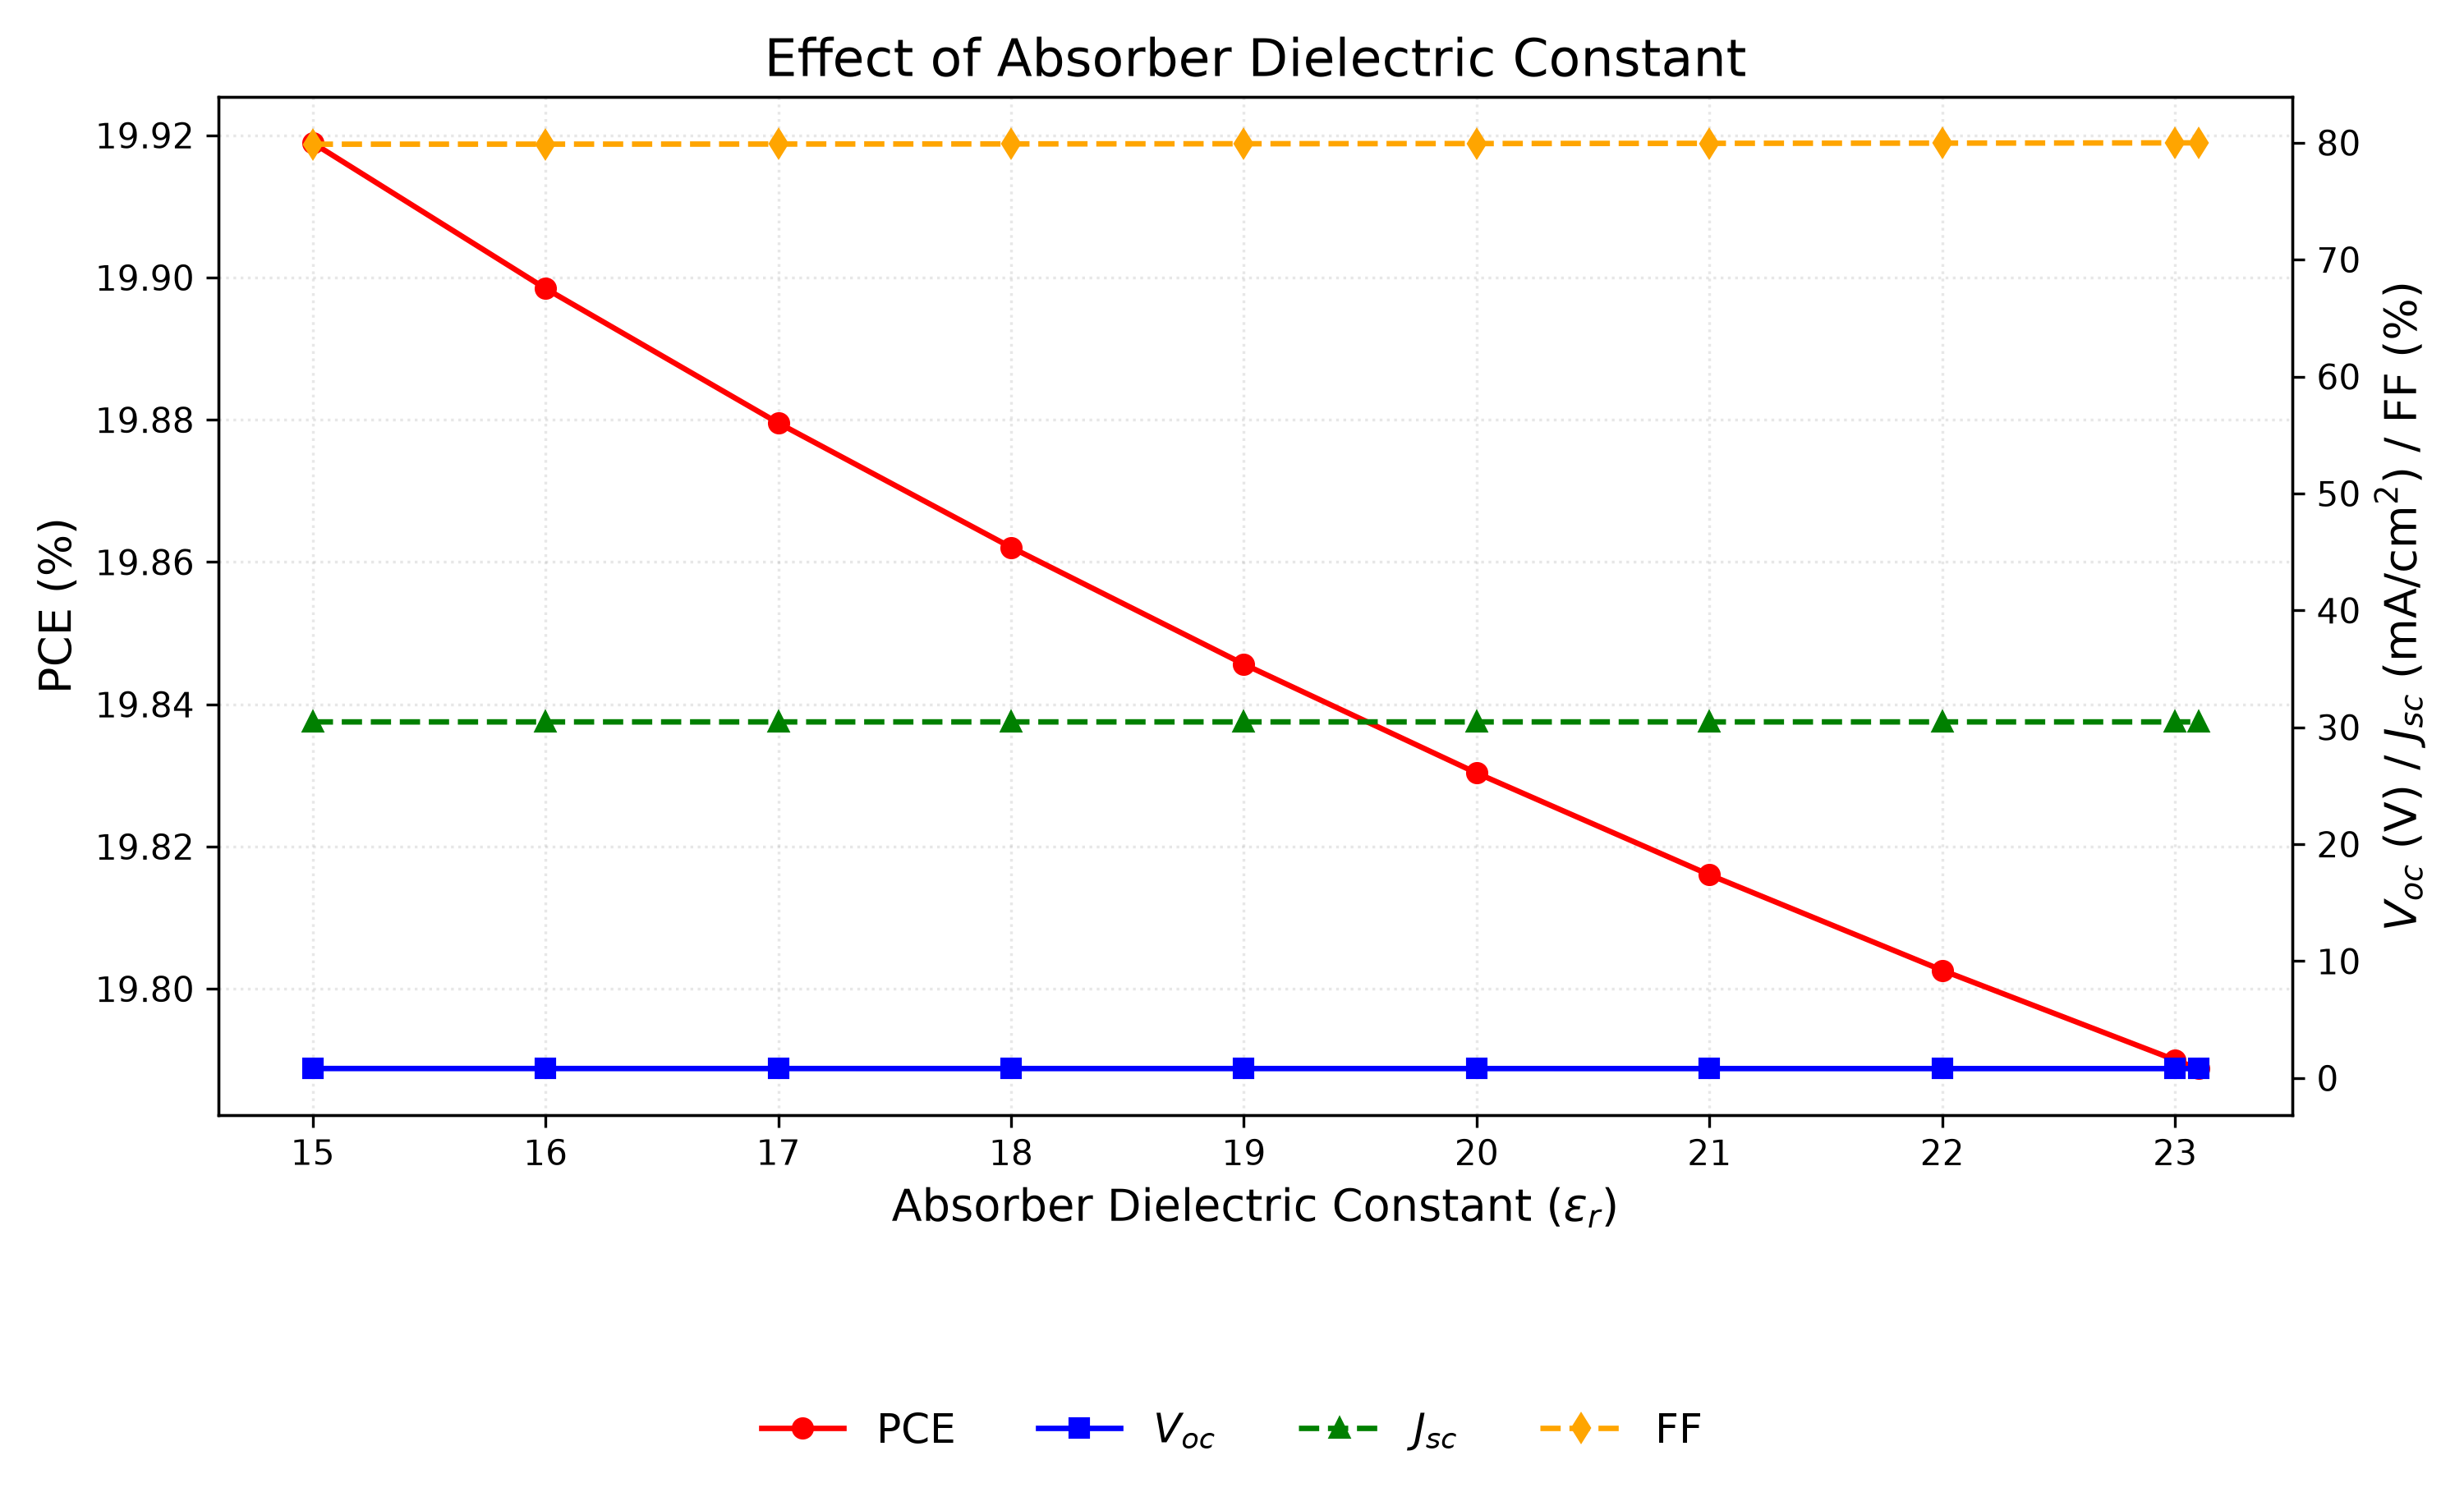
\includegraphics[width=0.85\linewidth]{figs/sup_fig5.png}
\caption{Fig.~S2: sweep over absorber dielectric constant.}\end{figure}

\subsection*{Electron affinity (Fig.~S3)}
Peak at $\chi=3.9$\,eV (19.79\%); 4.2\,eV costs $V_{\mathrm{OC}}$ 0.812$\rightarrow$0.710\,V at flat $J_{\mathrm{SC}}$.
\begin{figure}[H]\centering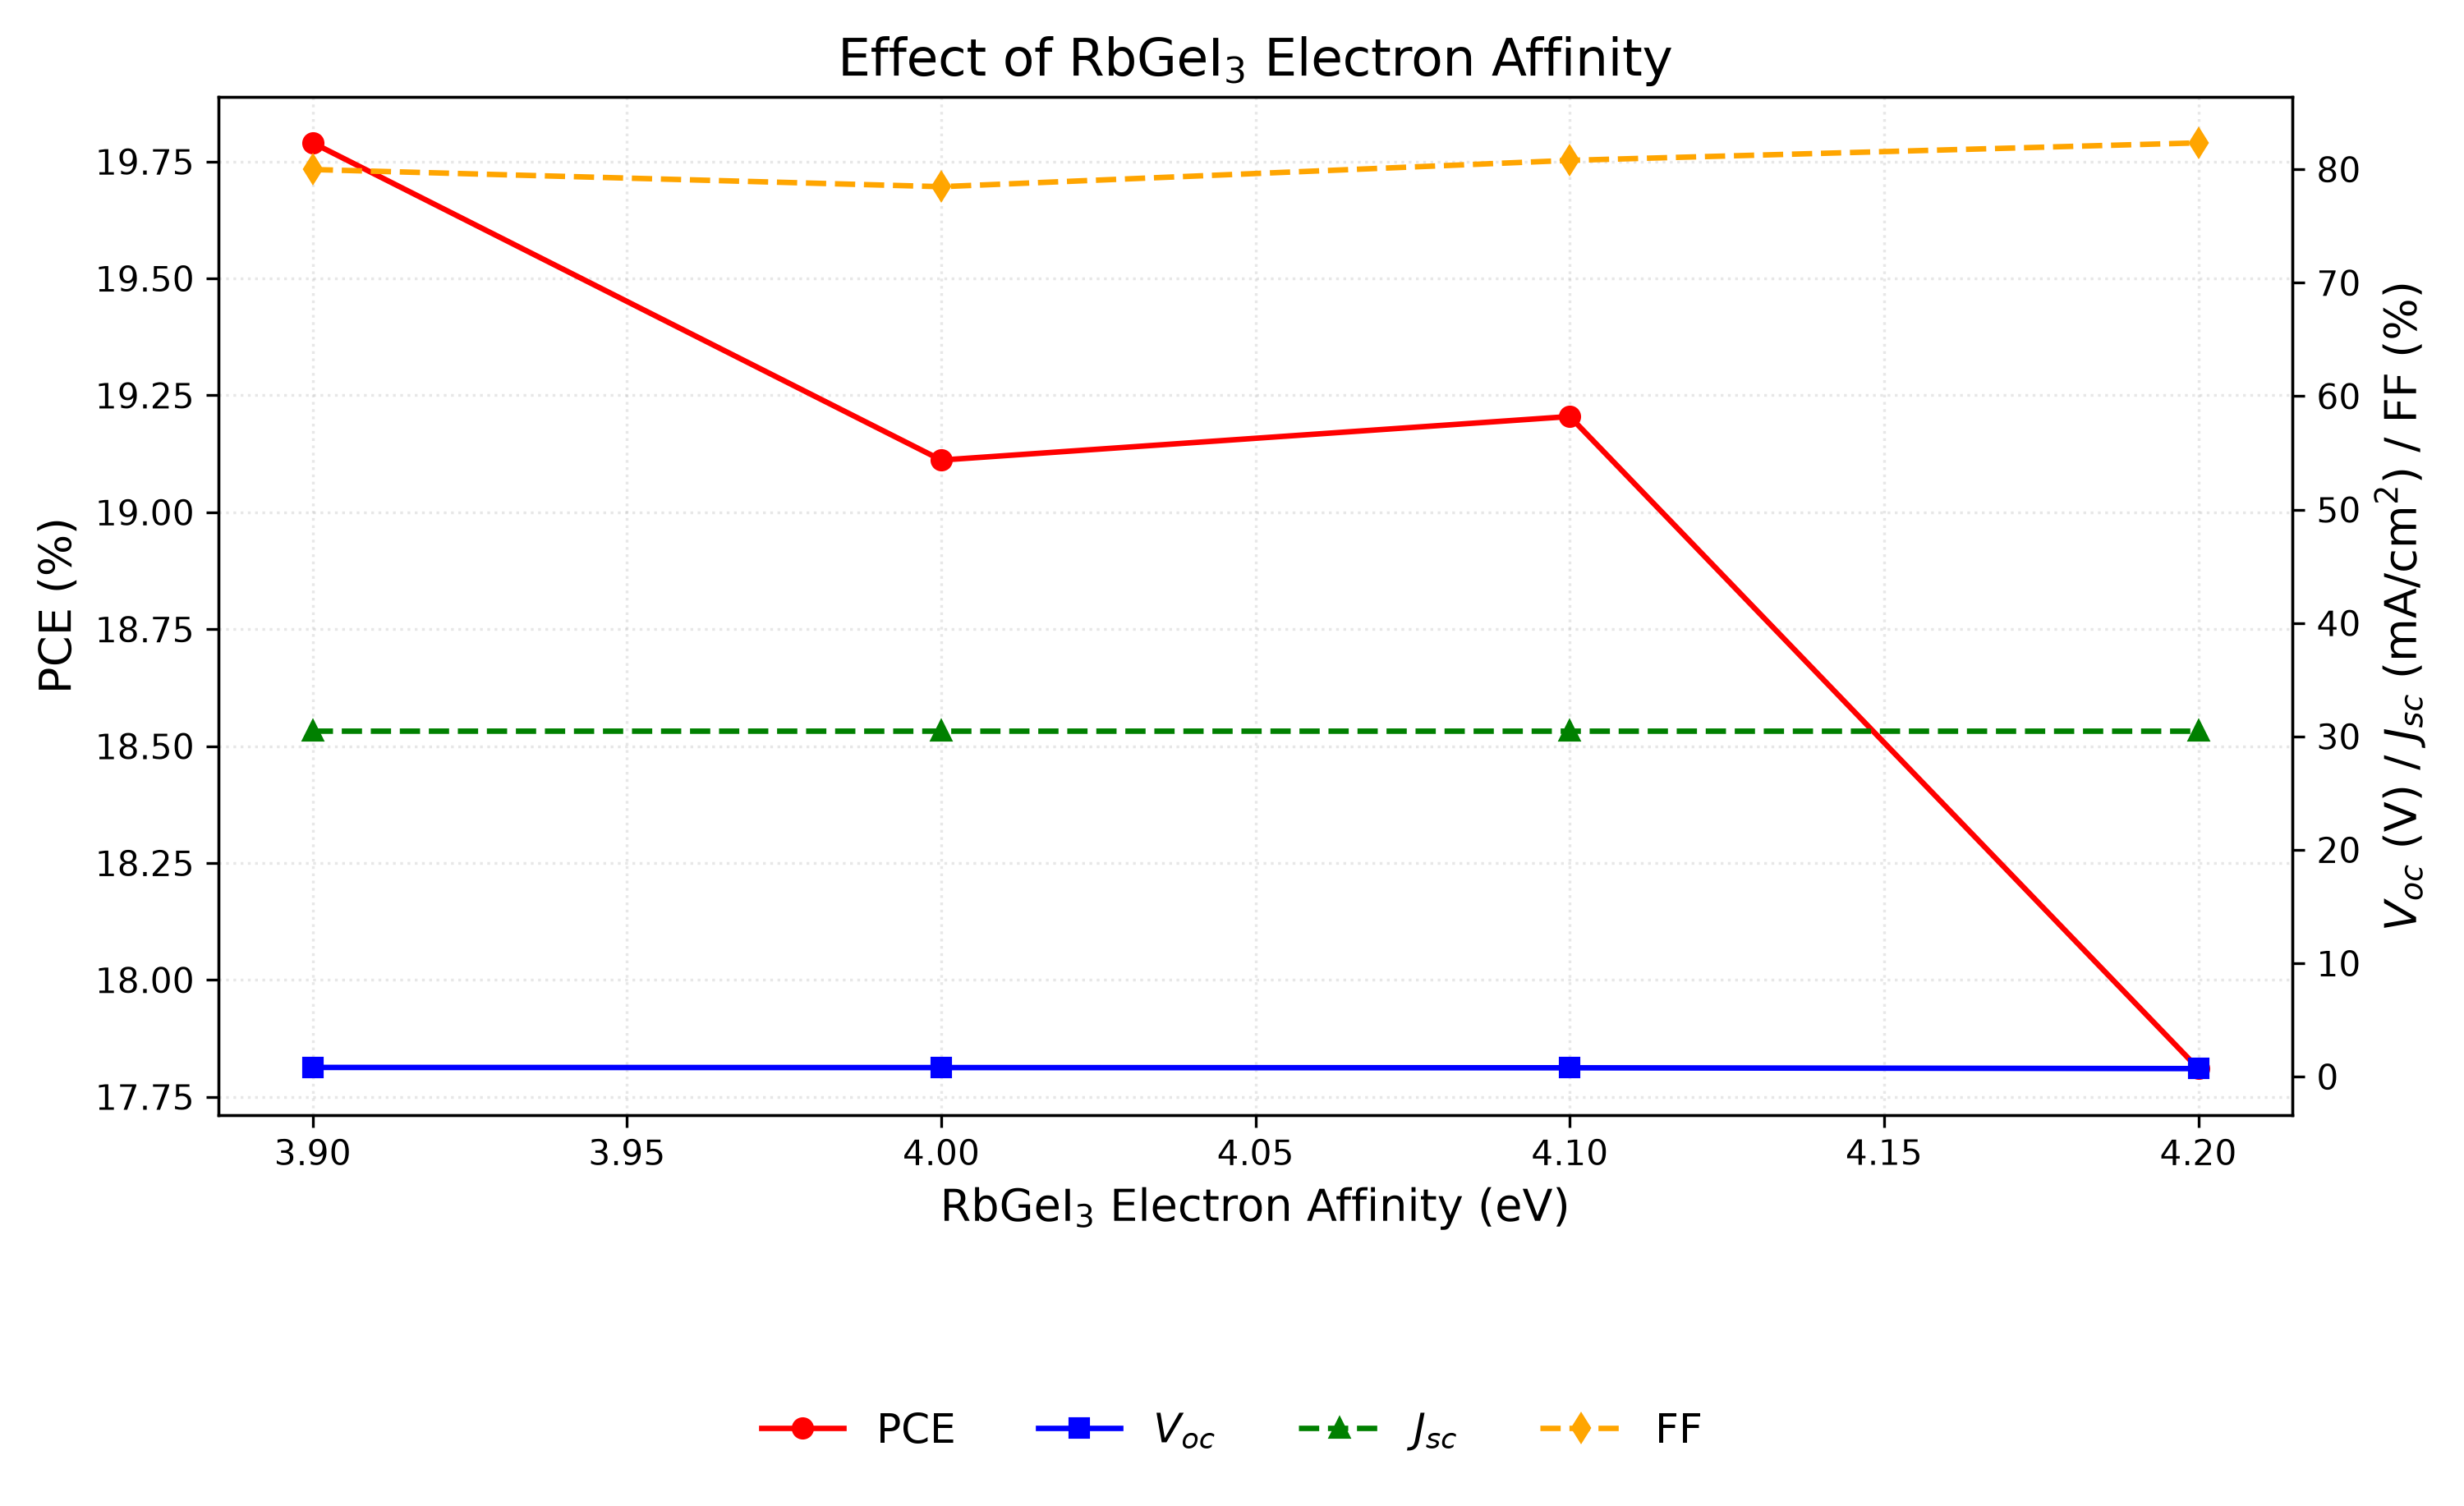
\includegraphics[width=0.85\linewidth]{figs/sup_fig6.png}
\caption{Fig.~S3: sweep over absorber electron affinity.}\end{figure}

\subsection*{TiO$_{2}$/RbGeI$_{3}$ interface (Fig.~S4)}
The performance cliff: $10^{12}$$\rightarrow$$10^{18}$\,cm$^{-2}$ sends PCE 21.04$\rightarrow$8.40\%; $10^{14}$\,cm$^{-2}$ adopted as the fabricable target.
\begin{figure}[H]\centering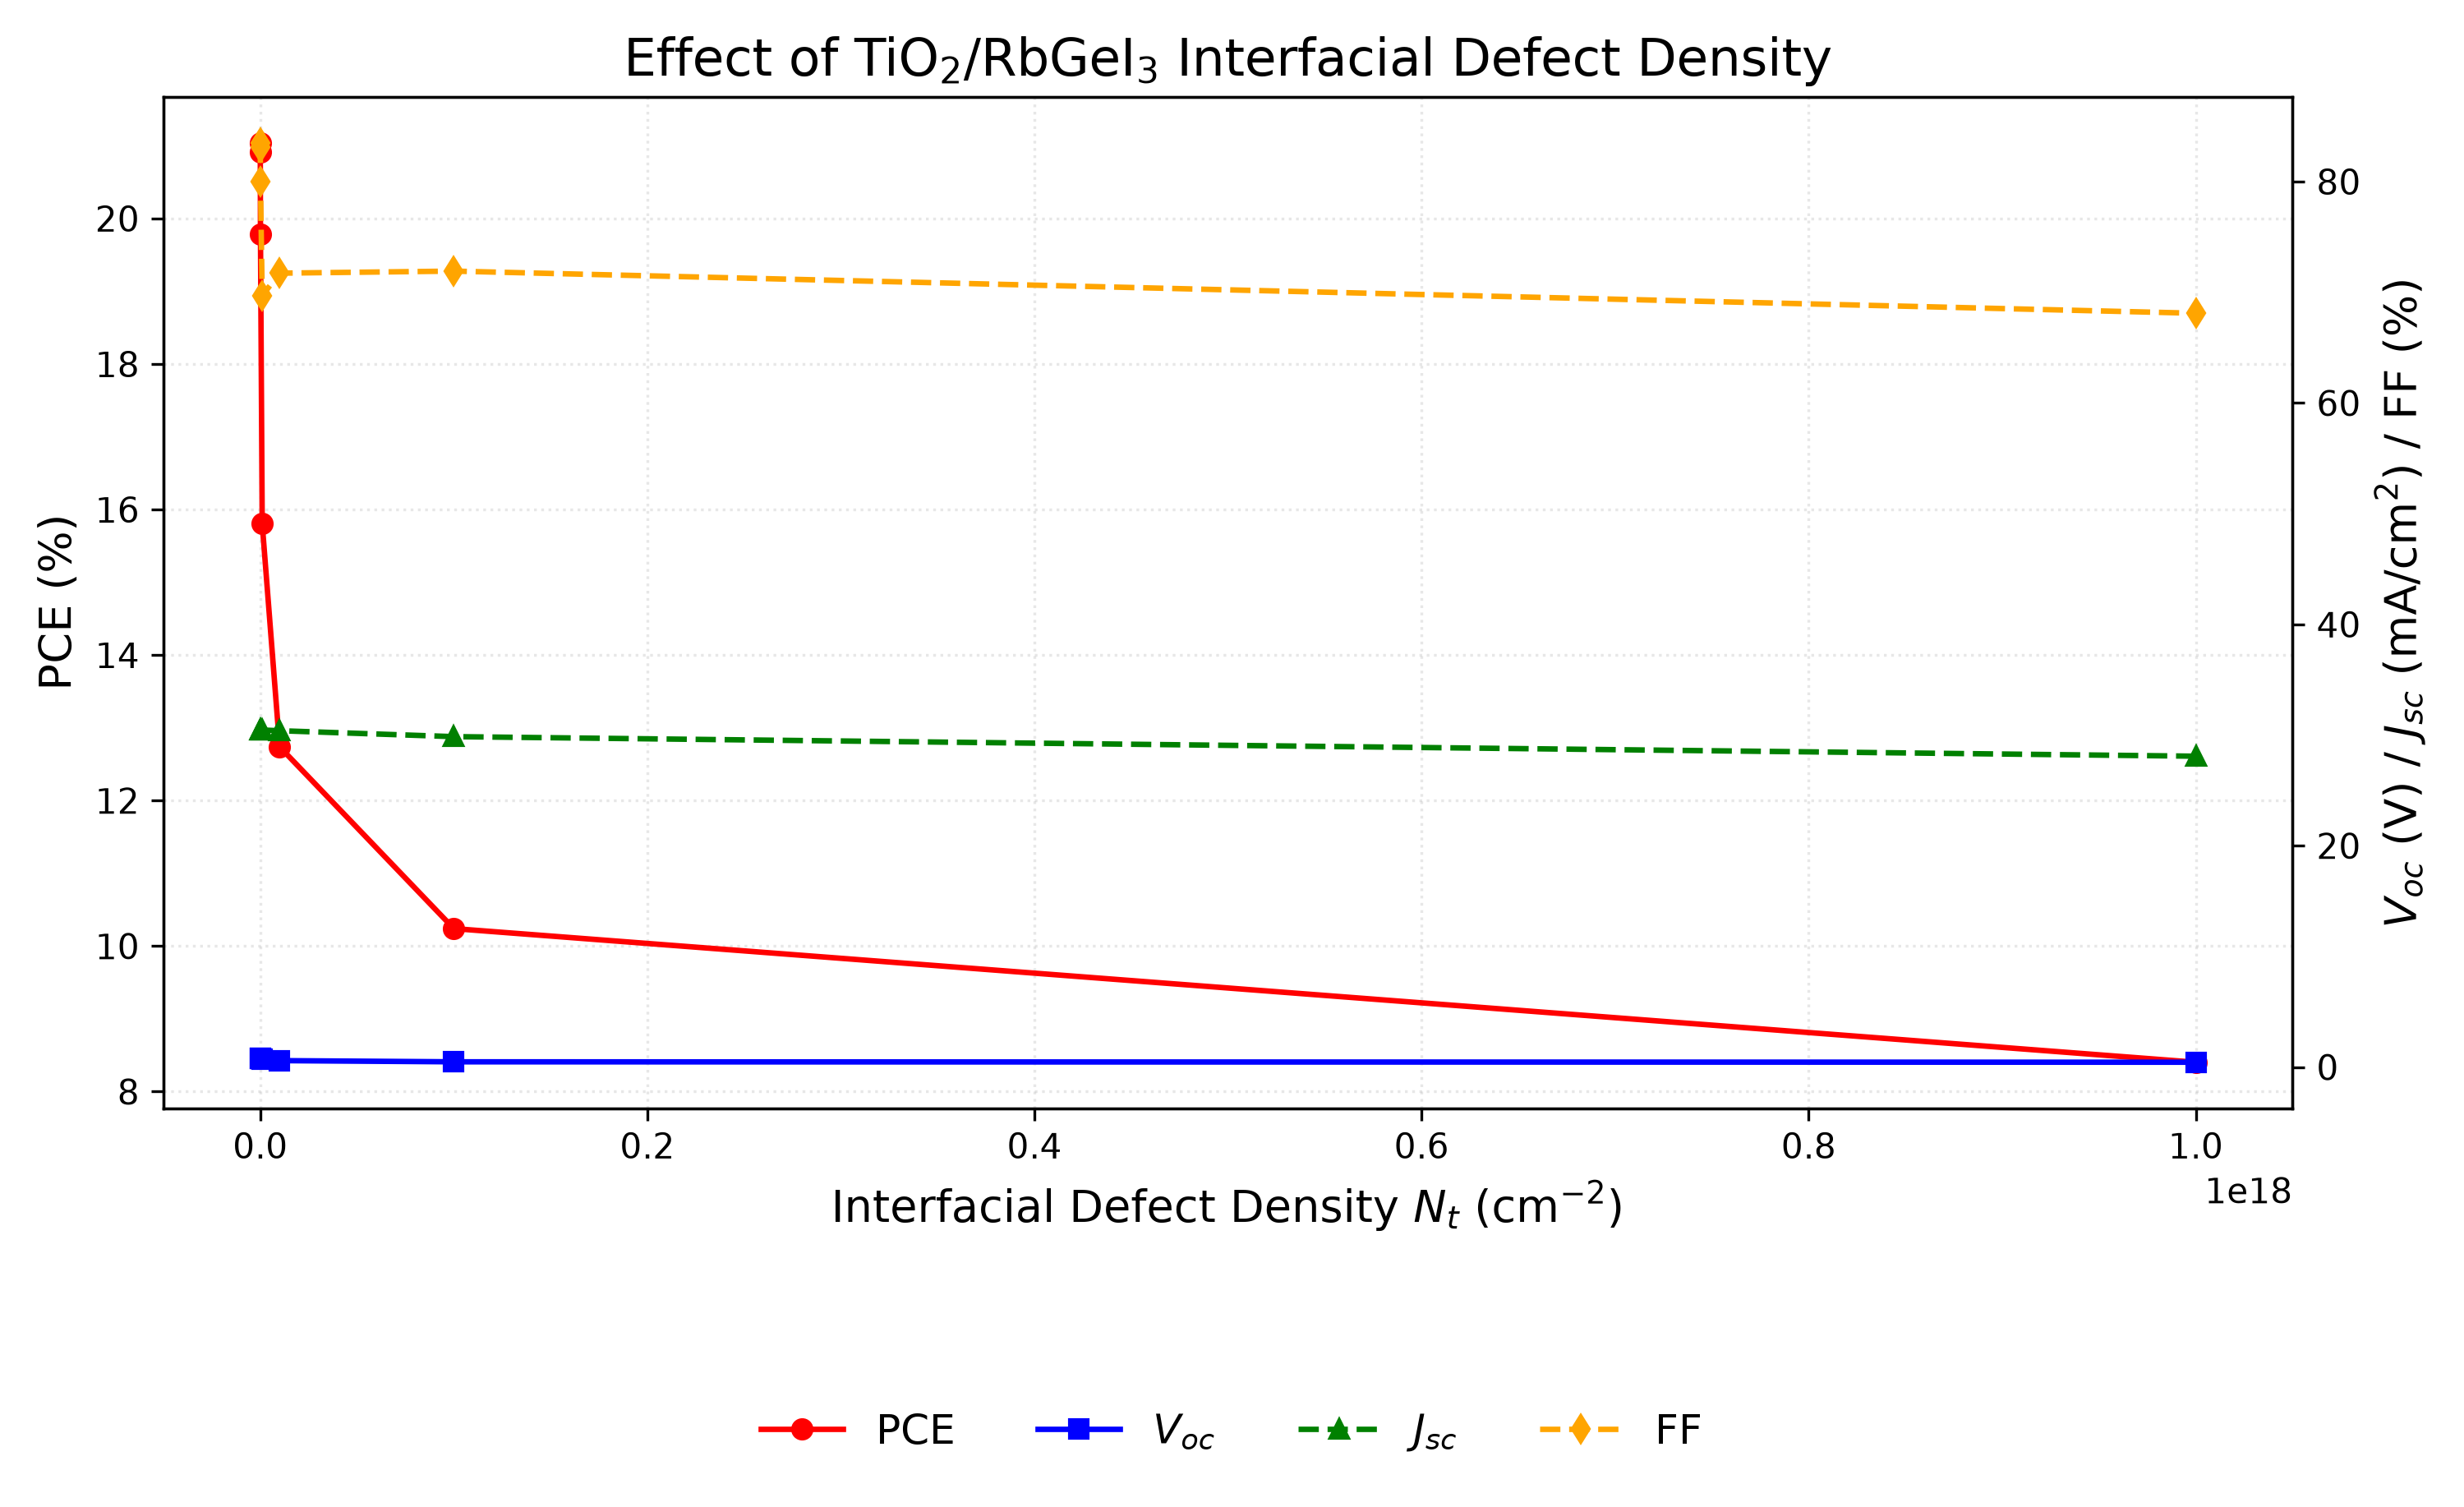
\includegraphics[width=0.85\linewidth]{figs/sup_fig7.png}
\caption{Fig.~S4: TiO$_{2}$/RbGeI$_{3}$ interfacial defect sweep.}\end{figure}

\subsection*{RbGeI$_{3}$/CuI interface (Fig.~S5)}
Far more tolerant (19.79$\rightarrow$18.19\%); the electron side pins the limit. $10^{14}$\,cm$^{-2}$ adopted for consistency.
\begin{figure}[H]\centering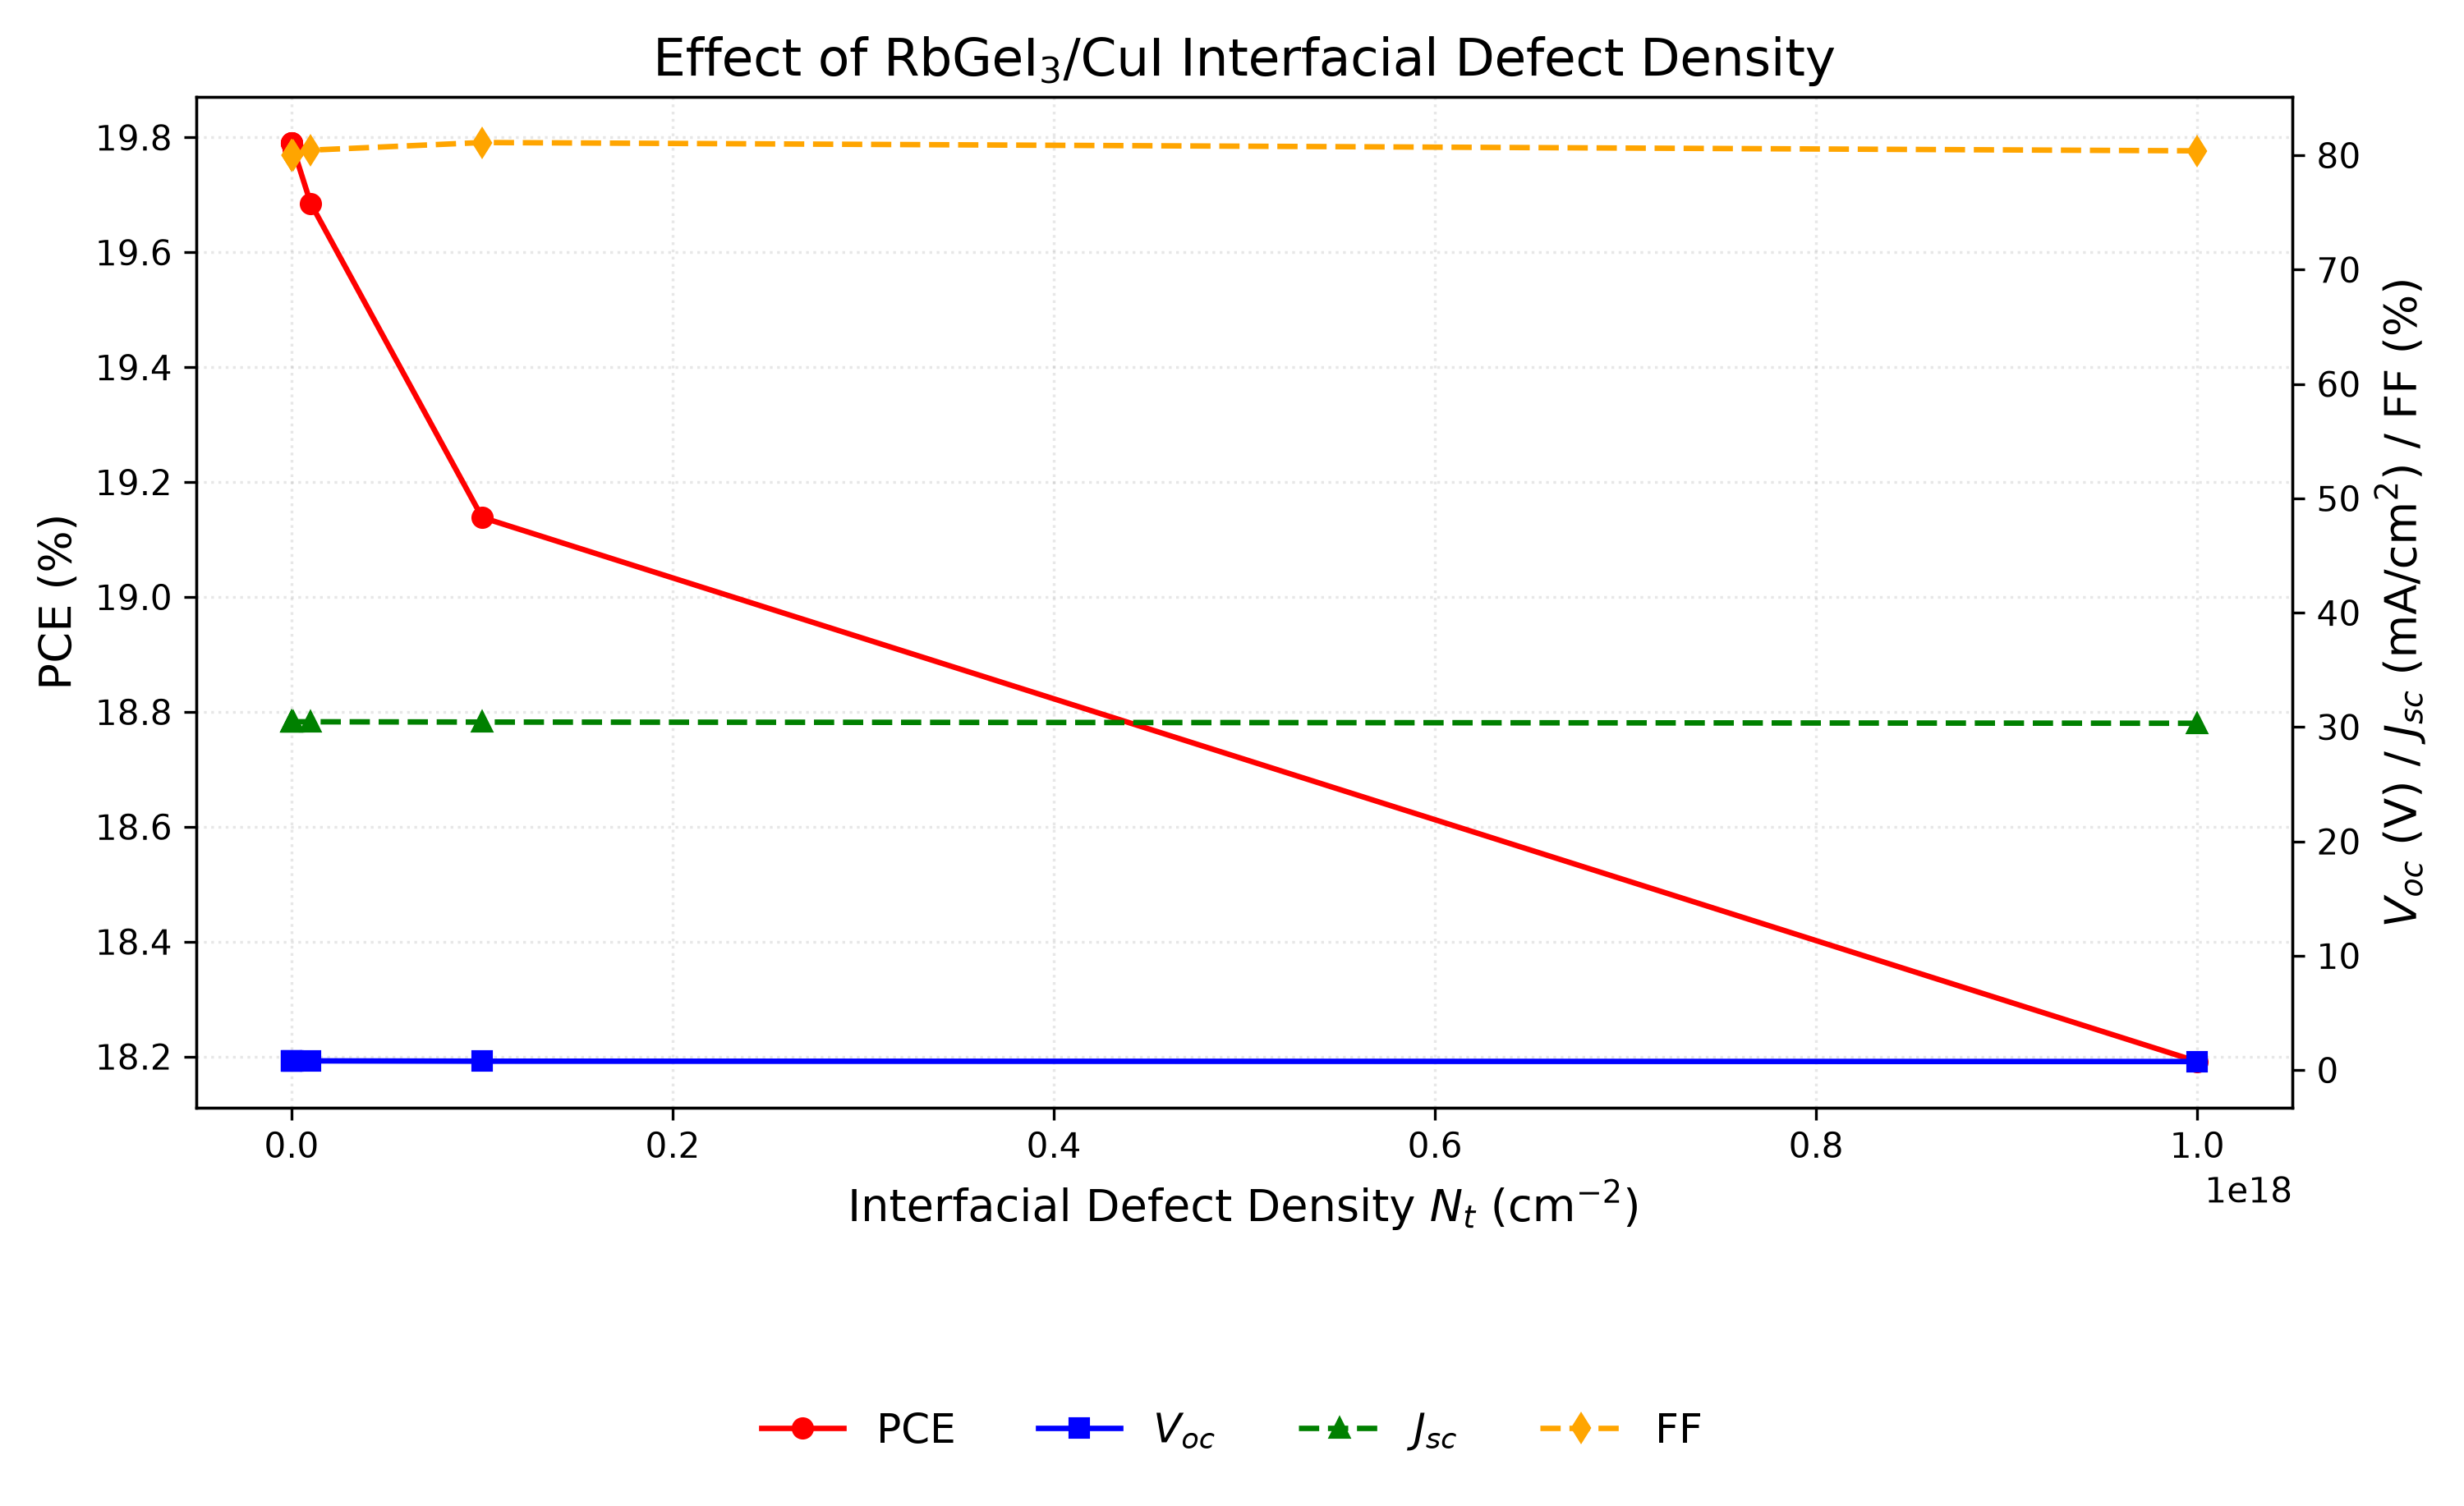
\includegraphics[width=0.85\linewidth]{figs/sup_fig8.png}
\caption{Fig.~S5: RbGeI$_{3}$/CuI interfacial defect sweep.}\end{figure}

\subsection*{Bandgap (Fig.~S6)}
$V_{\mathrm{OC}}$ 0.840$\rightarrow$1.002\,V vs $J_{\mathrm{SC}}$ 33.59$\rightarrow$20.30\,mA/cm$^{2}$ over 1.3--1.7\,eV; optimum 1.4\,eV sits 0.06\,eV from the SQ optimum ($\approx$1.34\,eV); $\lambda_{c}=1240/1.4\approx886$\,nm matches the QE edge.
\begin{figure}[H]\centering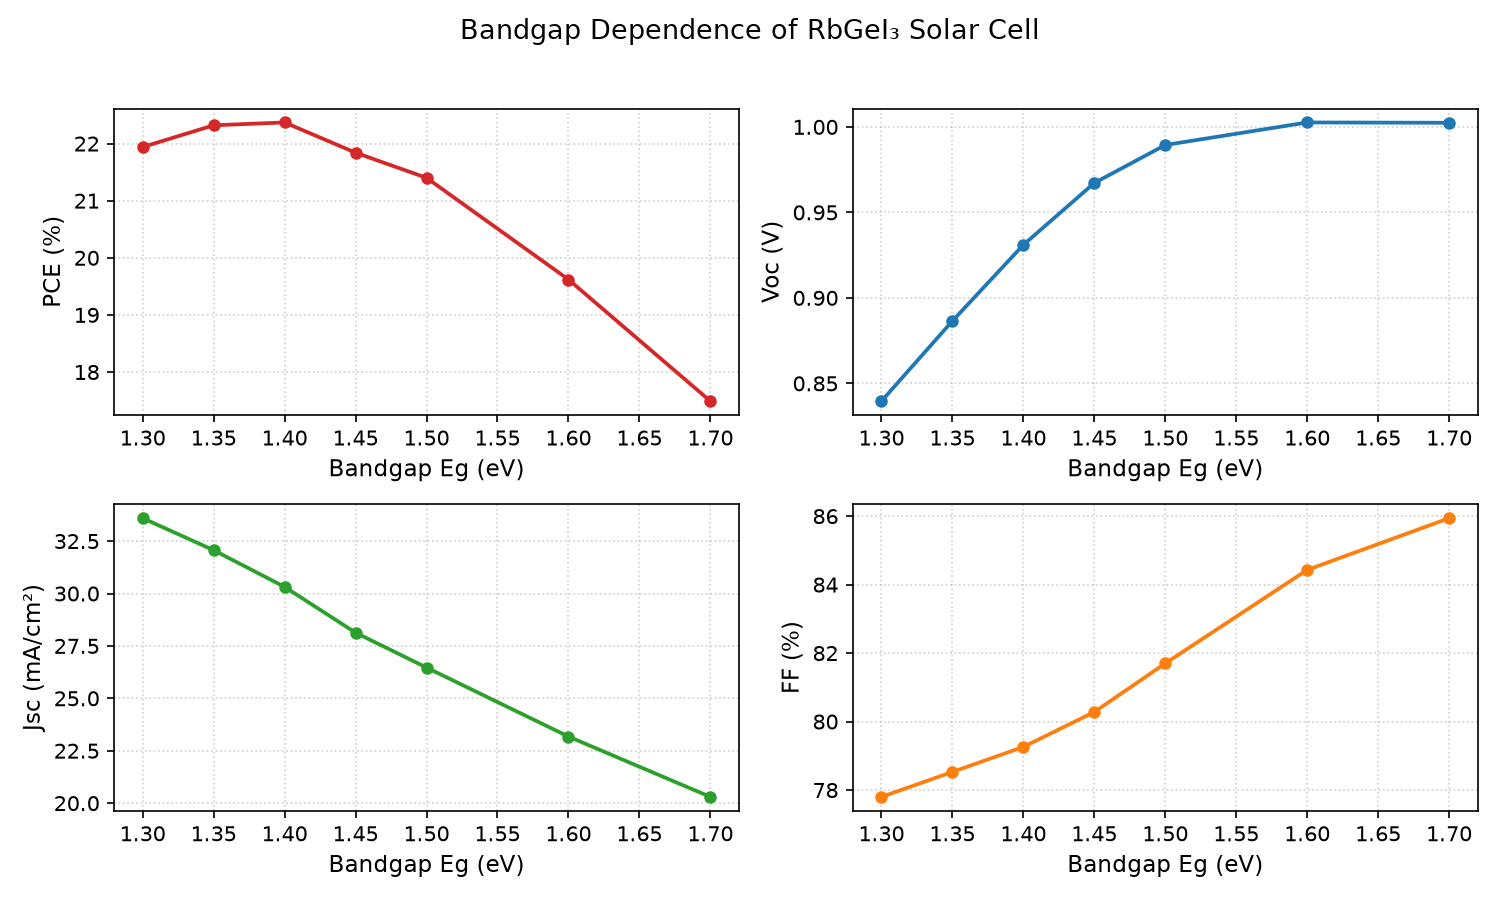
\includegraphics[width=0.85\linewidth]{figs/sup_fig9.png}
\caption{Fig.~S6: sweep over absorber bandgap.}\end{figure}

\subsection*{TiO$_{2}$ thickness (Fig.~S7)}
Best at the thinnest ETL (21.12\% at 10\,nm); thicker layers add resistance and parasitic absorption.
\begin{figure}[H]\centering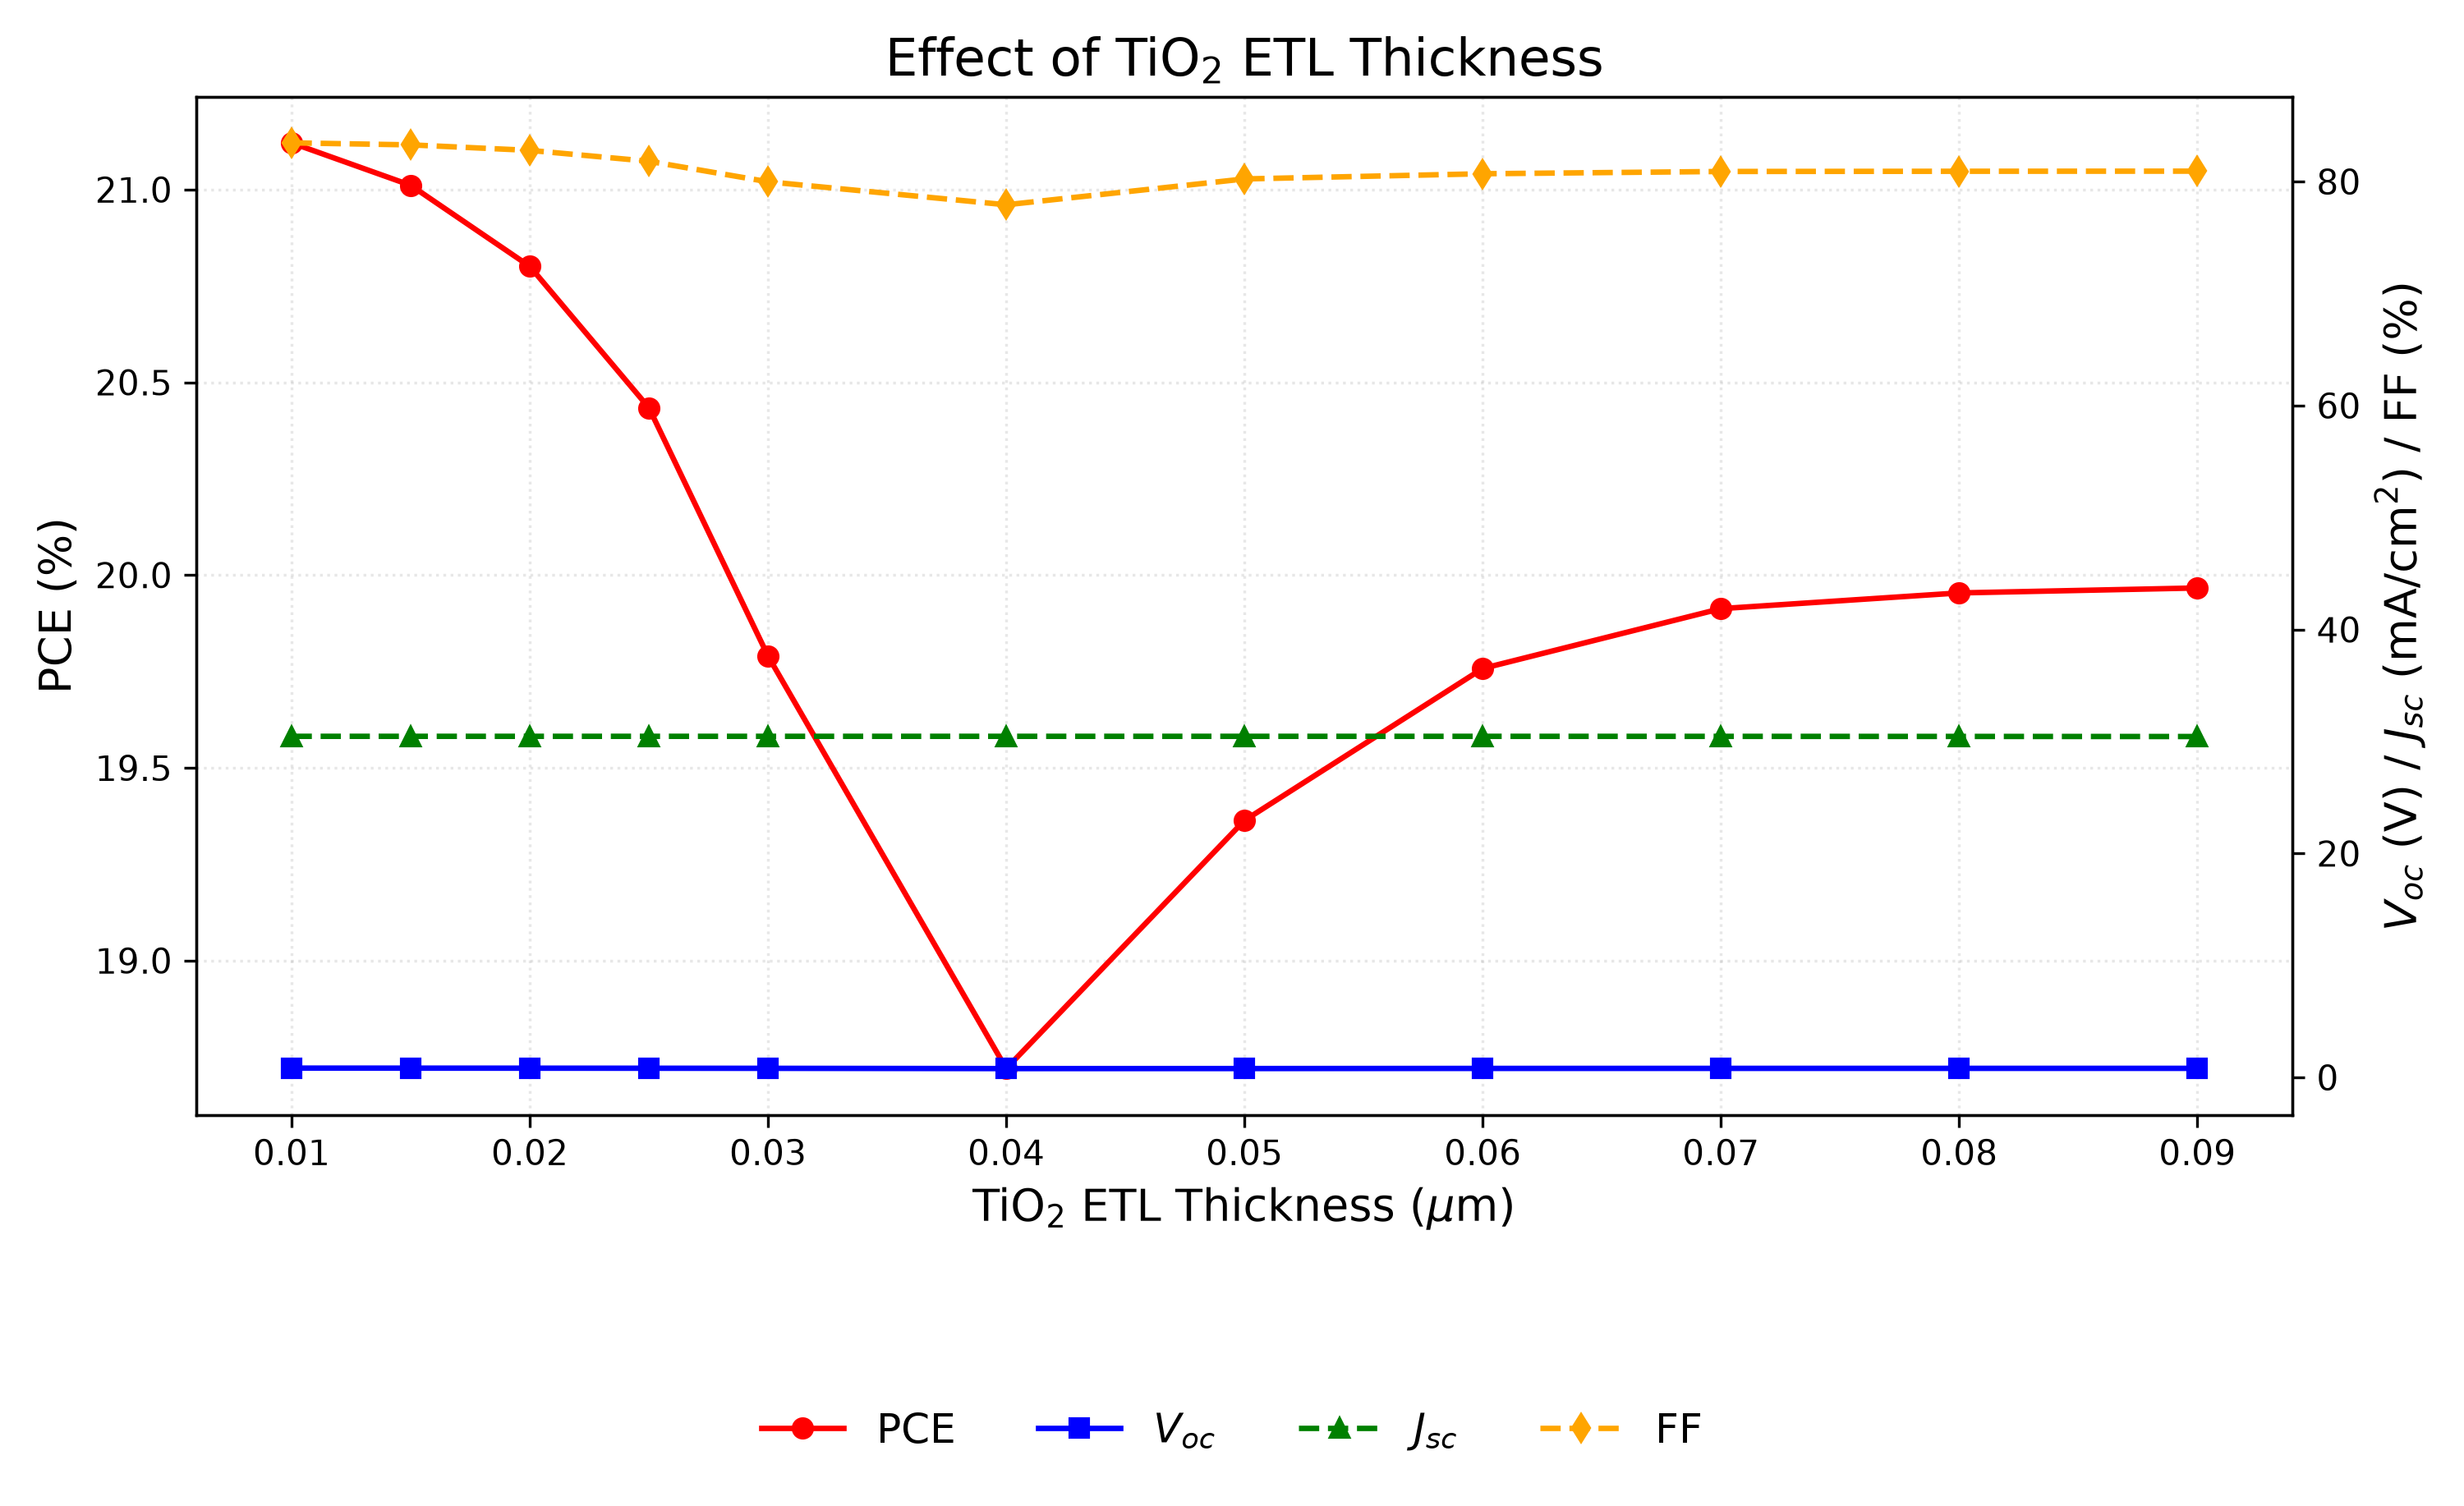
\includegraphics[width=0.85\linewidth]{figs/sup_fig10.png}
\caption{Fig.~S7: sweep over TiO$_{2}$ ETL thickness.}\end{figure}

\subsection*{CuI thickness (Fig.~S8)}
Flat within 0.002\,pp over 0.1--1.9\,$\mu$m; 100\,nm minimizes material use.
\begin{figure}[H]\centering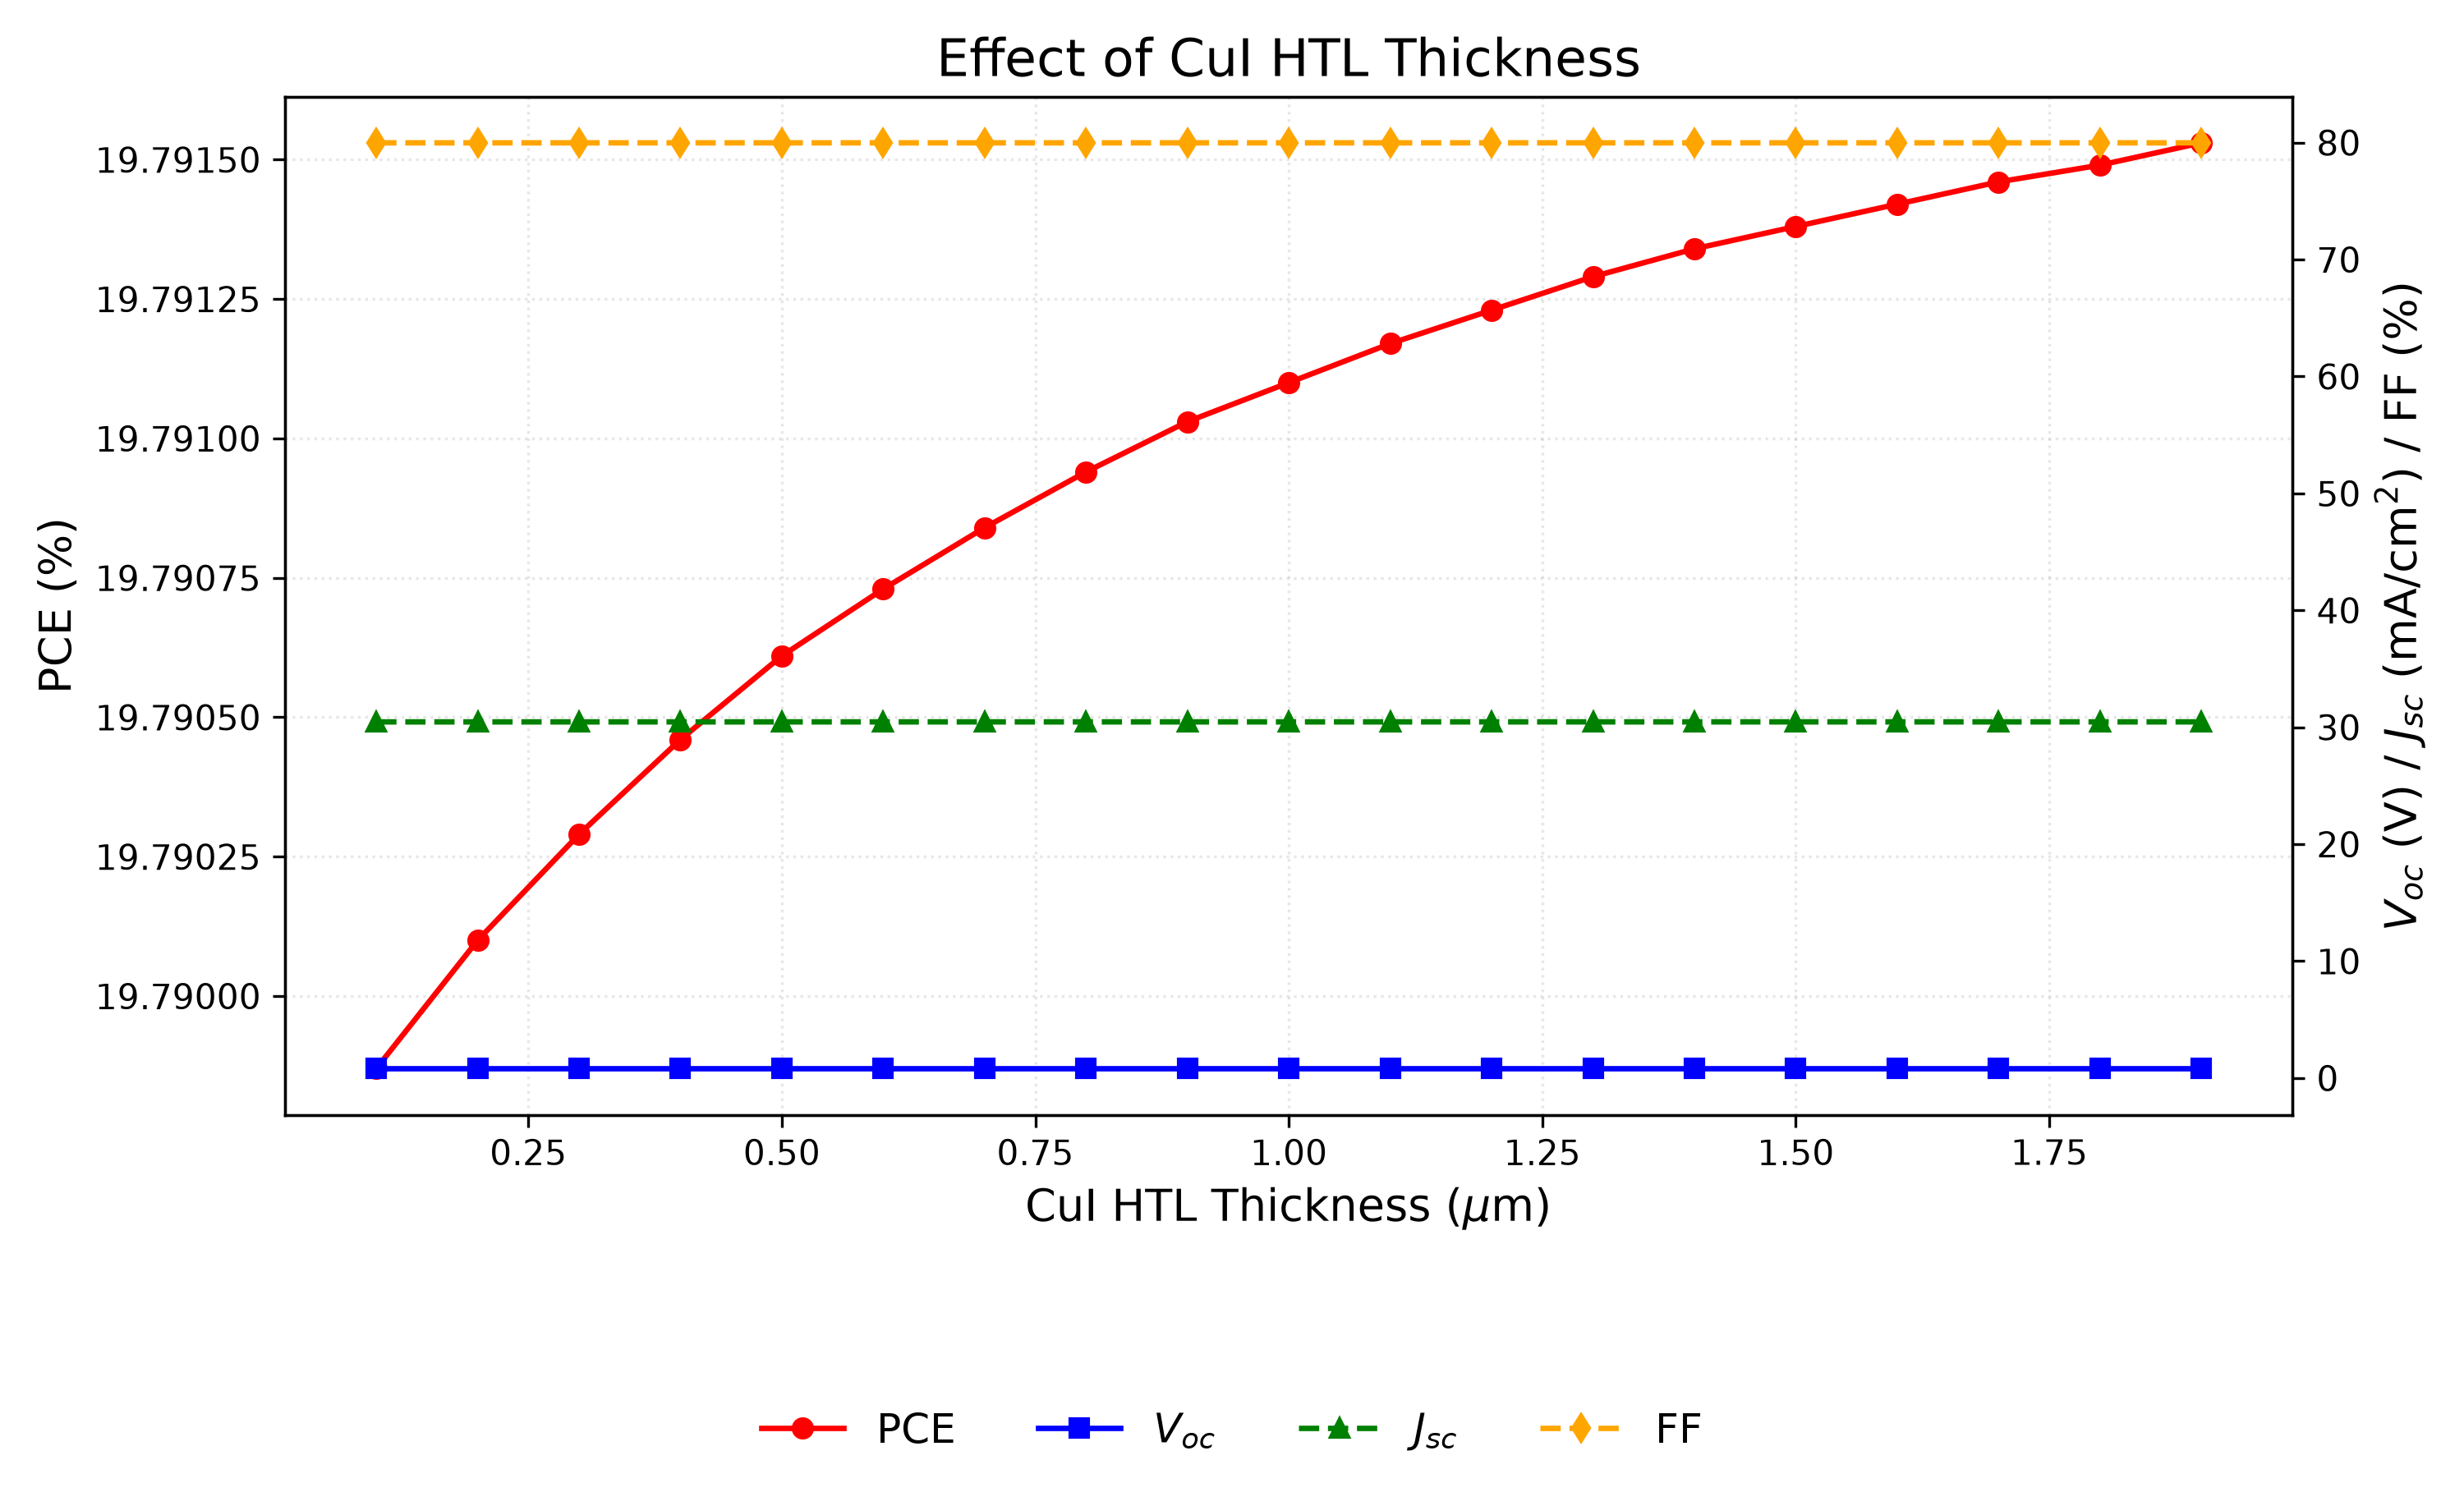
\includegraphics[width=0.85\linewidth]{figs/sup_fig11.png}
\caption{Fig.~S8: sweep over CuI HTL thickness.}\end{figure}

\subsection*{$N_{C}$ and $N_{V}$ (Figs.~S9--S10)}
Lower densities raise $V_{\mathrm{OC}}$ at flat $J_{\mathrm{SC}}$; both carried at $10^{17}$\,cm$^{-3}$ (PCE 20.65\% and 23.54\% at the sweep bottoms).
\begin{figure}[H]\centering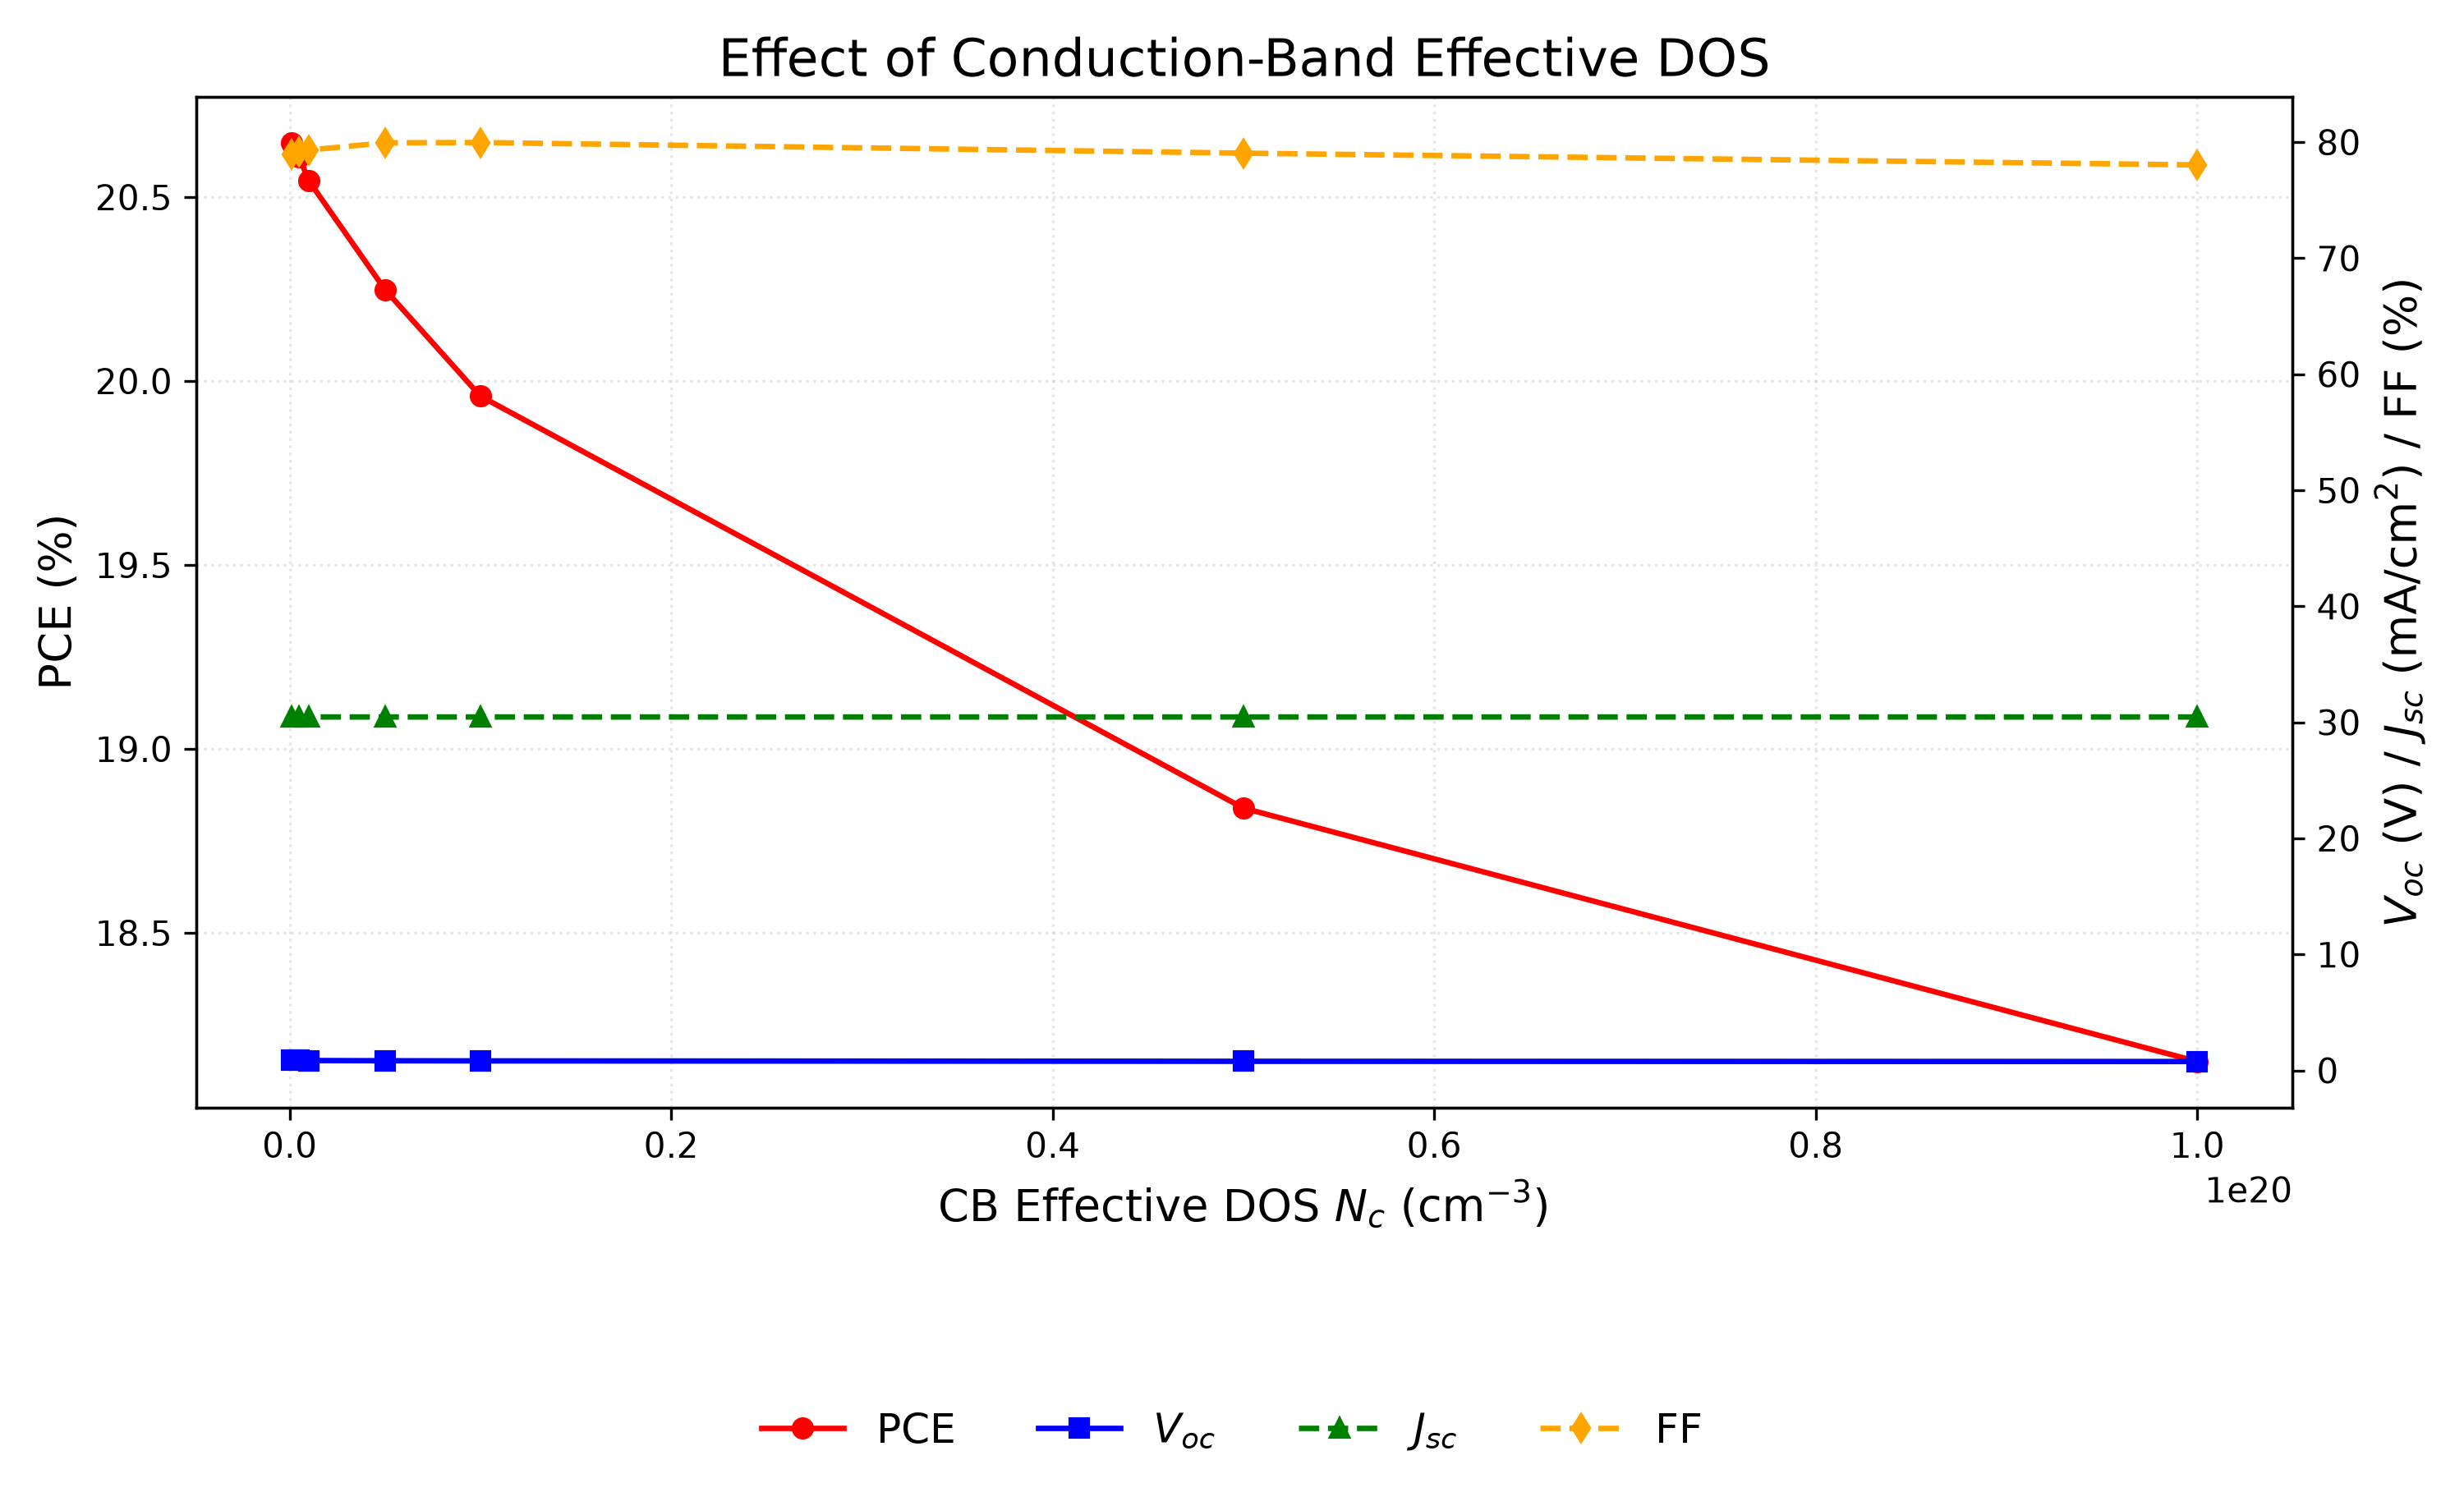
\includegraphics[width=0.85\linewidth]{figs/sup_fig12.png}
\caption{Fig.~S9: sweep over $N_{C}$.}\end{figure}
\begin{figure}[H]\centering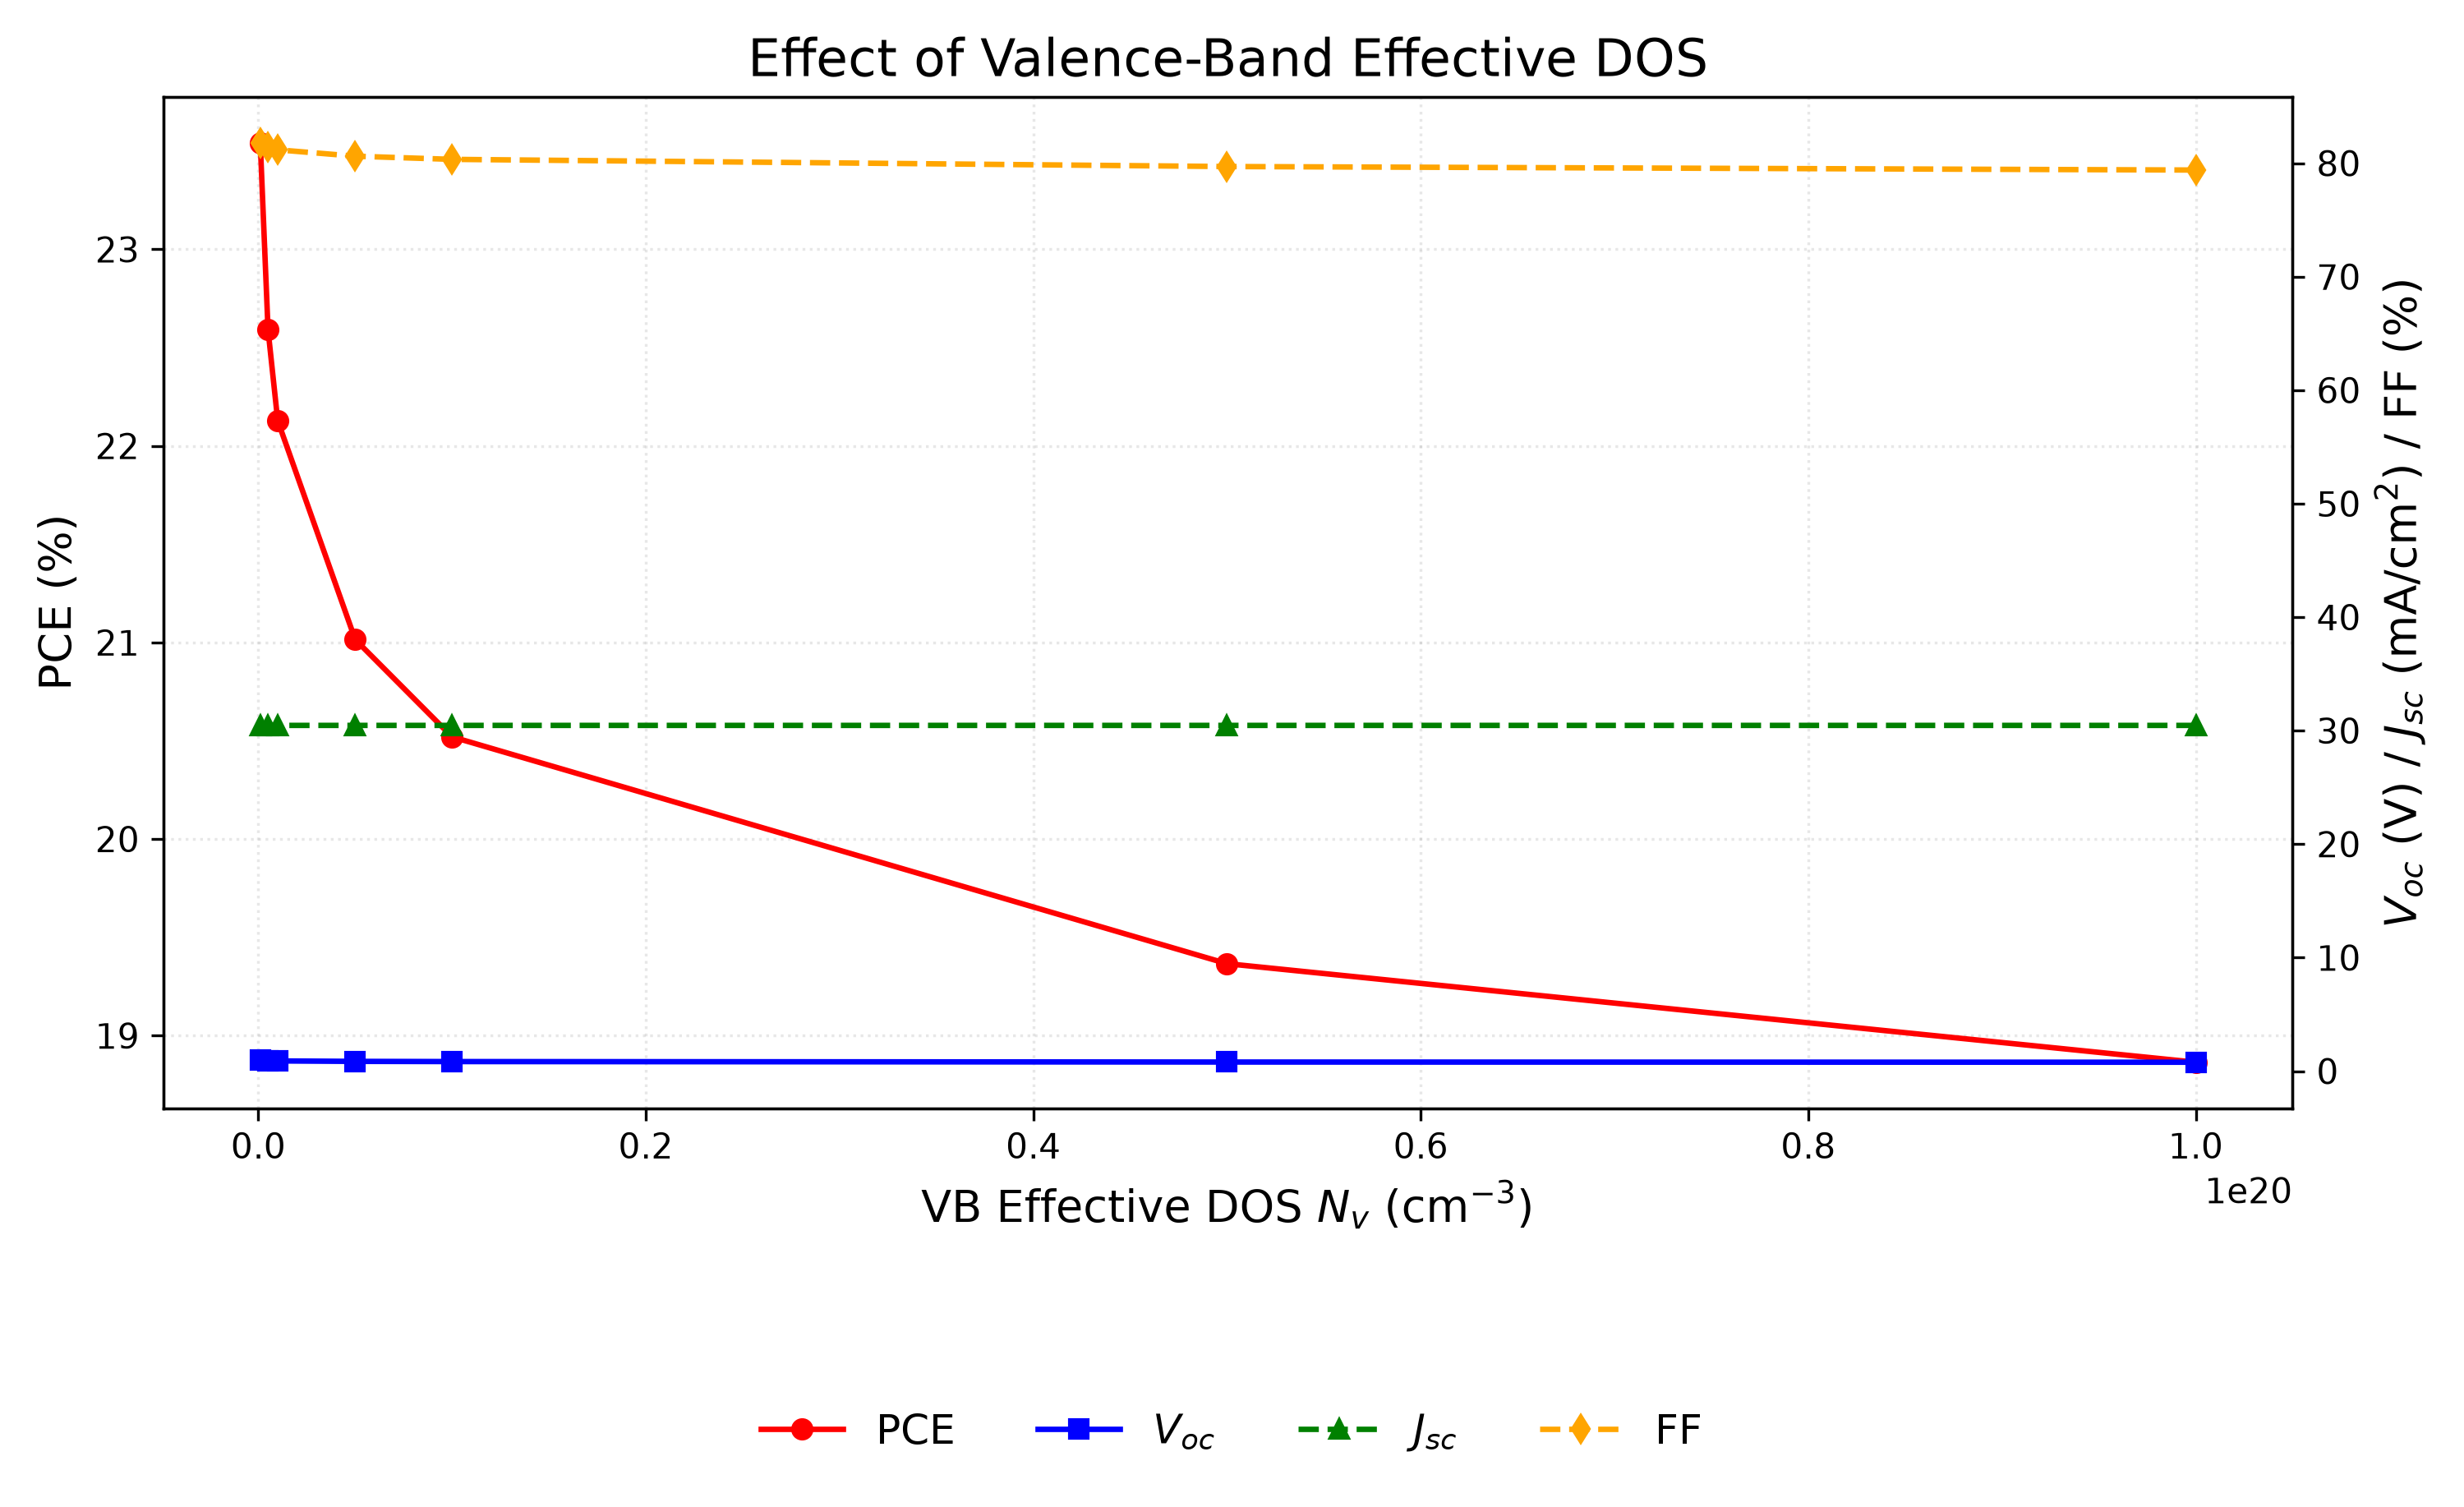
\includegraphics[width=0.85\linewidth]{figs/sup_fig13.png}
\caption{Fig.~S10: sweep over $N_{V}$.}\end{figure}

\section*{S2.\ Illumination and dark characteristics}
0.1--1.5\,suns: $J_{\mathrm{SC}}$ linear in intensity, $V_{\mathrm{OC}}$ logarithmic with ideality $n\approx1.2$ (Fig.~S11). Dark J--V rectifies $1.8\times10^{10}$ with leakage below $10^{-10}$\,A/cm$^{2}$ (Fig.~S12).
\begin{figure}[H]\centering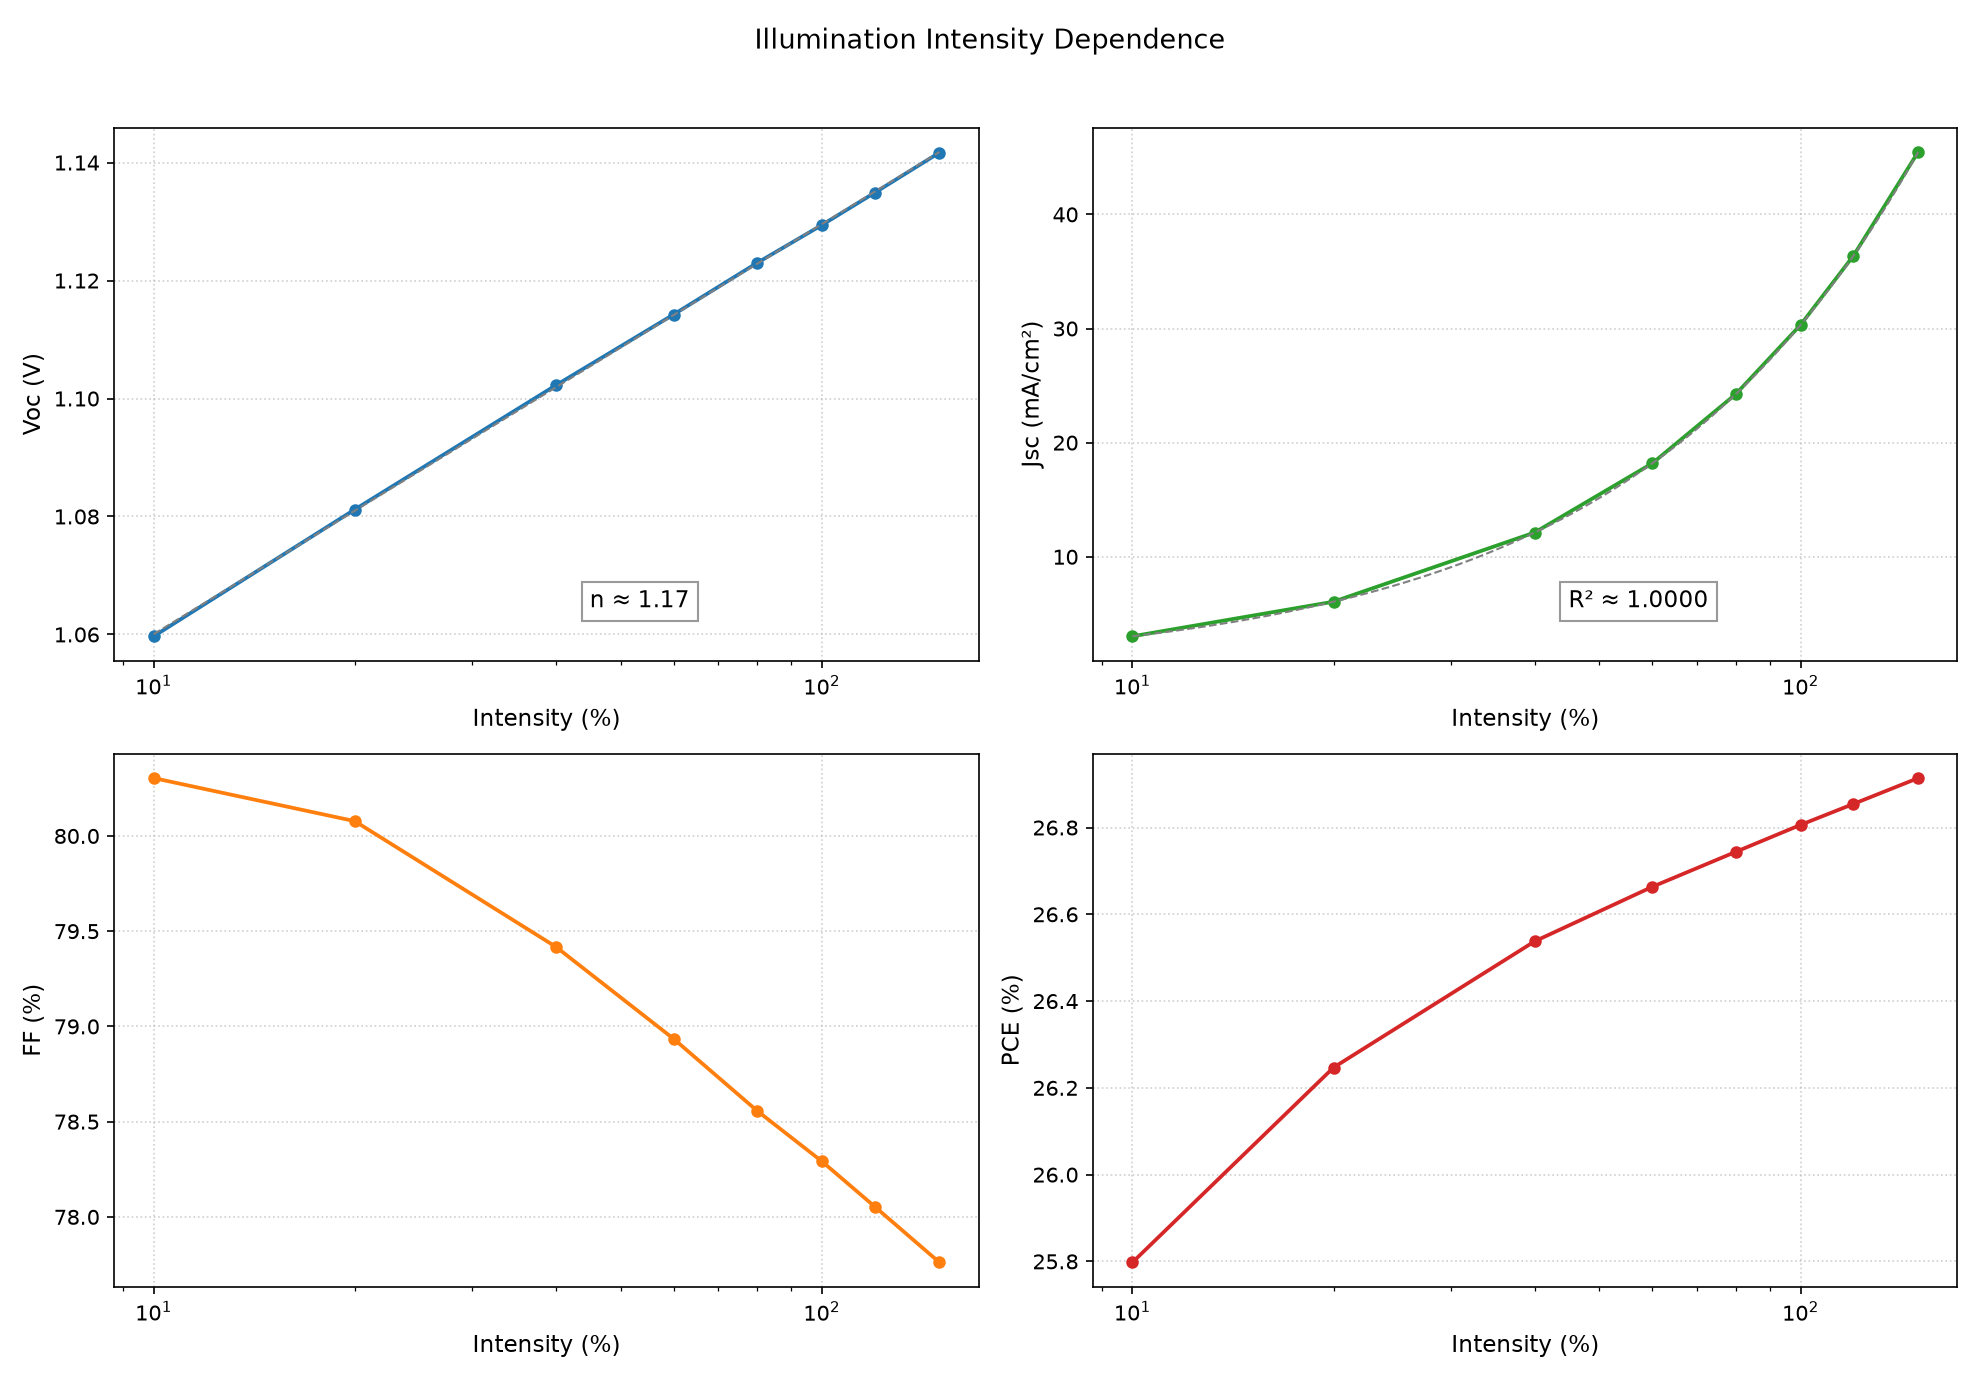
\includegraphics[width=0.85\linewidth]{figs/sup_fig18.png}
\caption{Fig.~S11: illumination dependence.}\end{figure}
\begin{figure}[H]\centering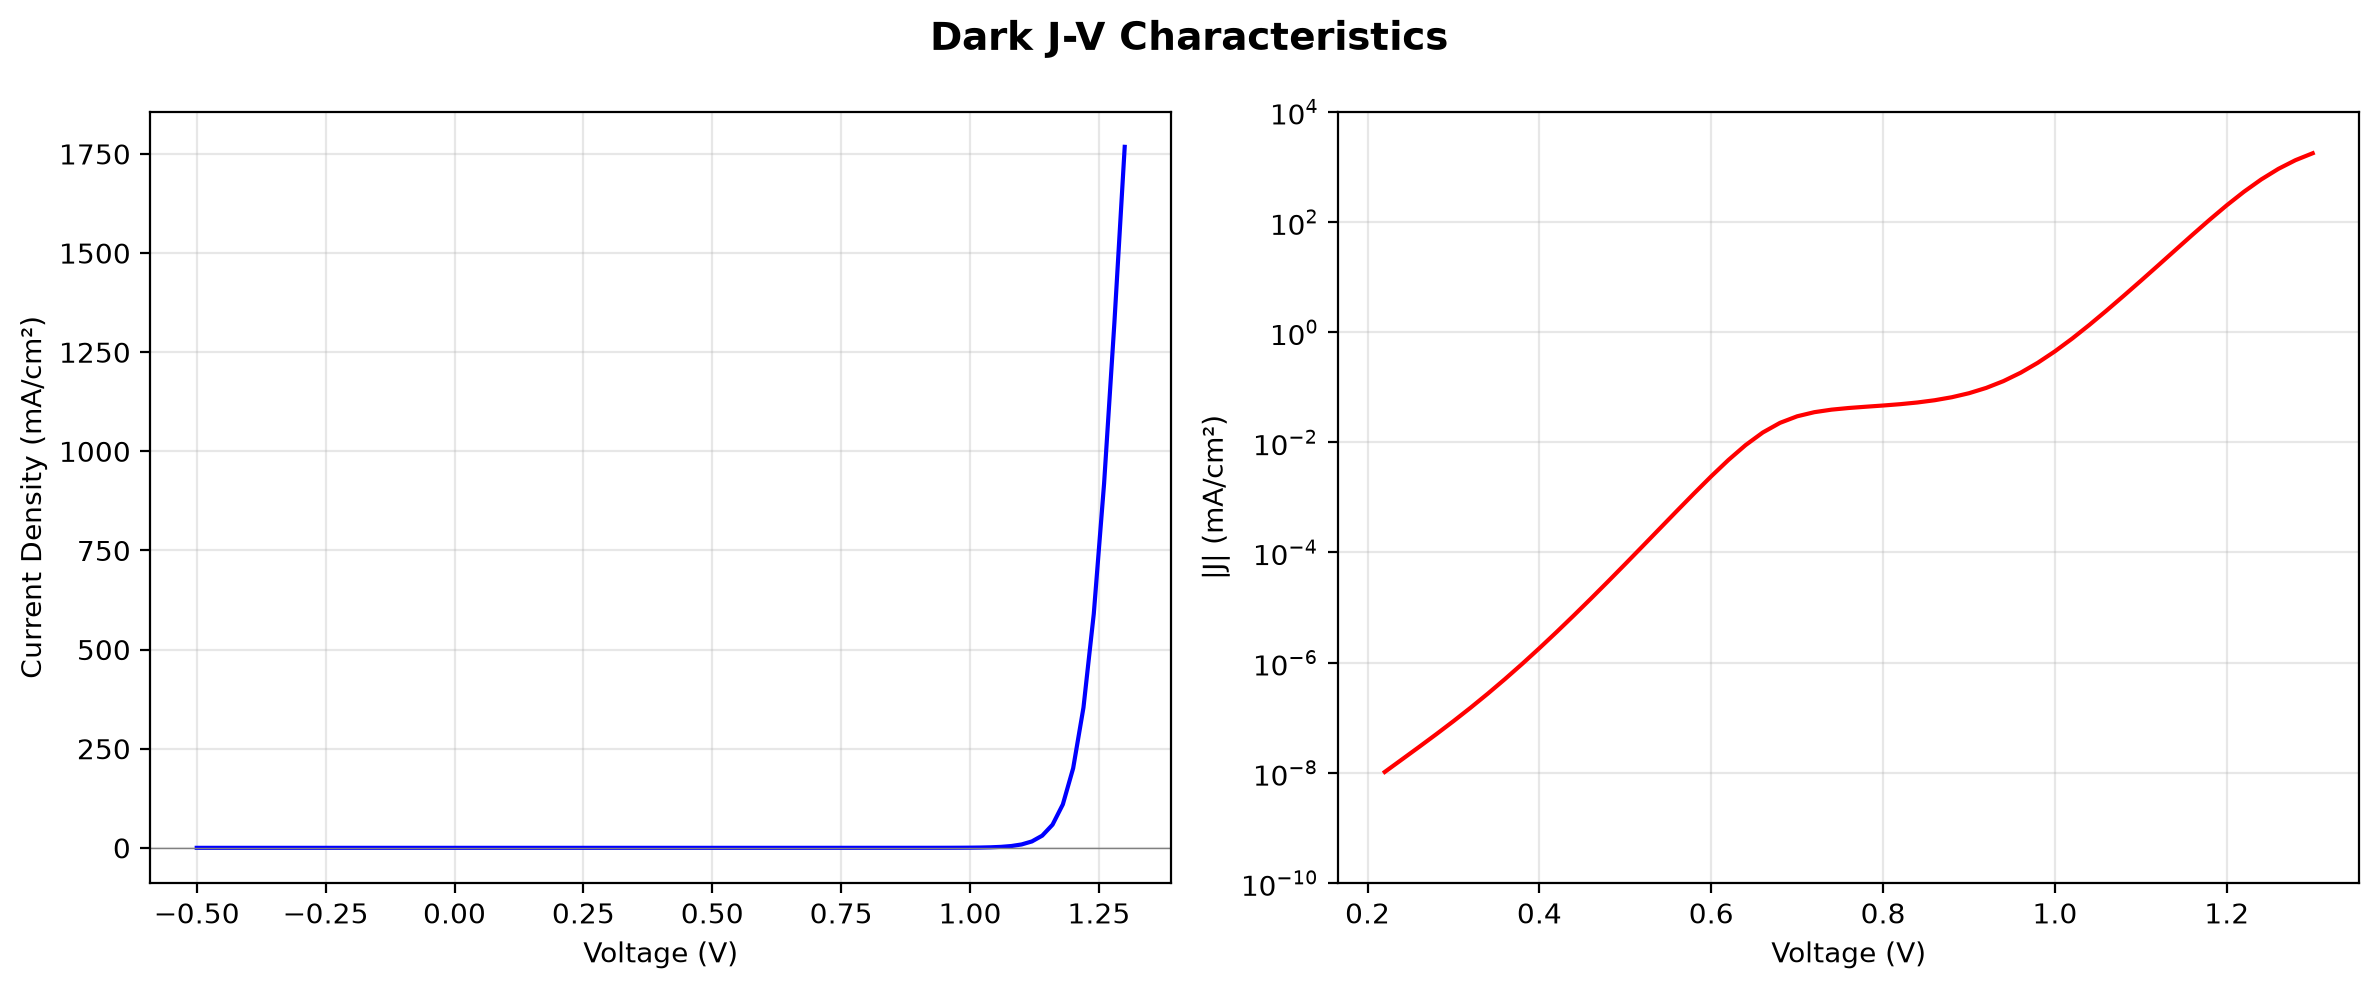
\includegraphics[width=0.85\linewidth]{figs/sup_fig19.png}
\caption{Fig.~S12: dark J--V.}\end{figure}

\section*{S3.\ Tables}
\begin{table}[H]\centering{\small\setlength{\tabcolsep}{3pt}
\begin{tabularx}{\textwidth}{Xccc}
\hline
Study & Device & PCE (\%) & Key limitation\\
\hline
Pindolia 2022 & FTO/TiO$_{2}$/RbGeI$_{3}$/NiO/Ag & 9.77 & Modest baseline; oxidation unaddressed\\
Saikia 2022 & FTO/TiO$_{2}$/CsGeI$_{3}$/CuI/Au & 10.80 & No multi-HTL comparison\\
Loumachi 2024 & ITO/C$_{60}$/RbGeI$_{3}$/CBTS/Ag & 27.21 & Interface defects unaddressed\\
Raj 2025 & FTO/TiO$_{2}$/RbGeI$_{3}$/PEDOT:PSS/Au & 18.60 & Organic HTL stability\\
Pathak 2026 & FTO/TiO$_{2}$/RbGeI$_{3}$/Spiro/Au & 26.47 & Single ETL/HTL; oxidation unaddressed\\
Dash 2025 & DFT+SCAPS RbGeX$_{3}$ & 25.76 & Material-level focus\\
\hline
\end{tabularx}}
\caption{Table~S1: SCAPS literature context for Ge-based cells.}\end{table}

\begin{table}[H]\centering{\footnotesize\setlength{\tabcolsep}{3pt}
\begin{tabularx}{\textwidth}{Xcccc}
\hline
Parameter & TiO$_{2}$ & FTO & RbGeI$_{3}$ & CuI\\
\hline
Thickness (nm) & 10 & 500 & 700 & 100\\
$E_{g}$ (eV) & 3.2 & 3.2 & 1.4 & 3.1\\
$\chi$ (eV) & 4.0 & 4.4 & 3.9 & 2.1\\
$\epsilon_{r}$ & 9 & 9 & 15 & 6.5\\
$N_{C}$ (cm$^{-3}$) & $2\times10^{18}$ & $2.2\times10^{18}$ & $1\times10^{17}$ & $2.8\times10^{19}$\\
$N_{V}$ (cm$^{-3}$) & $1.8\times10^{19}$ & $1.8\times10^{19}$ & $1\times10^{17}$ & $1\times10^{19}$\\
$\mu_{e}$ (cm$^{2}$/Vs) & 20 & 20 & 28.6 & 100\\
$\mu_{p}$ (cm$^{2}$/Vs) & 10 & 10 & 27.3 & 43.9\\
$N_{D}$ (cm$^{-3}$) & $9\times10^{16}$ & $1\times10^{19}$ & $1\times10^{9}$ & 0\\
$N_{A}$ (cm$^{-3}$) & 0 & 0 & $1\times10^{9}$ & $1\times10^{18}$\\
$N_{t}$ (cm$^{-3}$) & $1\times10^{15}$ & $1\times10^{14}$ & $1\times10^{14}$ & $1\times10^{14}$\\
\hline
\end{tabularx}}
\caption{Table~S2: consolidated (optimized) layer parameters. Interfaces: $10^{14}$\,cm$^{-2}$ both junctions (Table~S3 in prior submission).}\end{table}

\begin{table}[H]\centering{\small\setlength{\tabcolsep}{3pt}
\begin{tabularx}{\textwidth}{Xcccc}
\hline
BSF $d$ (nm) $\times$ $N_{A}$ (cm$^{-3}$) & $10^{17}$ & $10^{18}$ & $10^{19}$\\
\hline
30 & 28.61 & 30.07 & 30.35\\
50 & 28.74 & 30.07 & 30.35\\
80 & 28.76 & 30.08 & 30.35\\
100 & 28.76 & 30.08 & 30.35\\
\hline
\end{tabularx}}
\caption{Table~S3: BSF grid PCE (\%; \texttt{r6\_bsf\_sweep.json}, 12/12 converged). Doping dominates; thickness flat.}\end{table}

\begin{table}[H]\centering{\small\setlength{\tabcolsep}{3pt}
\begin{tabularx}{\textwidth}{Xcccc}
\hline
Waterfall node & $V_{\mathrm{OC}}$ (V) & $J_{\mathrm{SC}}$ & PCE$_{1\text{-sun}}$ (\%)\\
\hline
R0 ideal & 1.1298 & 30.32 & 26.81\\
R1 +radiative/Auger & 1.1294 & 30.32 & 26.79\\
R2 +10\% reflection & 1.1263 & 27.28 & 24.08\\
R3 +bulk $10^{15}$ & 1.1083 & 27.28 & 22.34\\
R4 +interfaces $10^{15}$ & 1.0473 & 27.26 & 20.80\\
R5full BSF + full realism & 1.0877 & 27.27 & 23.29\\
\hline
\end{tabularx}}
\caption{Table~S4: native loss waterfall (\texttt{r6\_realistic\_waterfall.json}).}\end{table}

\begin{thebibliography}{99}
\bibitem{s35} W.~Shockley and H.~J.~Queisser, J.\ Appl.\ Phys.\ 32, 510--519 (1961).
\bibitem{s36} S.~R\"uhle, Sol.\ Energy 130, 139--147 (2016).
\bibitem{s37} C.~H.~Henry, J.\ Appl.\ Phys.\ 51, 4494--4500 (1980).
\end{thebibliography}
\end{document}
